%  LaTeX support: latex@mdpi.com
%=================================================================
\documentclass[sustainability,article,submit,moreauthors,pdftex]{Definitions/mdpi}

\firstpage{1}
\makeatletter
\setcounter{page}{\@firstpage}
\makeatother
\pubvolume{xx}
\issuenum{1}
\articlenumber{5}
\pubyear{2026}
\copyrightyear{2026}
%\externaleditor{Academic Editor: name}
\history{Received: date; Accepted: date; Published: date}

%=================================================================
% Additional packages
\usepackage{multirow}
\usepackage{amsfonts}
\usepackage{bm}
\usepackage{algorithm}
\usepackage{algpseudocode}
\usepackage{graphicx}
\usepackage{xcolor}
\graphicspath{{../figures/}}

% Fix Algorithm font: force algorithmic environment to use document font (Palatino)
% instead of falling back to Computer Modern
\makeatletter
\renewcommand{\ALG@beginalgorithmic}{\normalfont}
\makeatother

%=================================================================
% Title
\Title{Dual-Camera LiDAR Fusion for Occlusion-Robust 3D Detection in Urban Driving Simulation}

% Authors
\Author{Xingnan Zhou $^{1}$ and Ciprian Alecsandru $^{1,}$*}

\AuthorNames{Xingnan Zhou, Ciprian Alecsandru}

% Affiliations
\address{%
$^{1}$ \quad Department of Building, Civil and Environmental Engineering, Concordia University, Montreal, QC H3G 1M8, Canada}

% Corresponding author
\corres{Correspondence: ciprian.alecsandru@concordia.ca (C.A.)}

%=================================================================
% Abstract
\abstract{Three-dimensional object detection from LiDAR point clouds is a cornerstone of autonomous driving perception, yet single-sensor systems remain vulnerable to false positives and occlusion in complex urban environments such as roundabouts and dense intersections. This paper proposes a dual-camera LiDAR fusion framework that combines 3D LiDAR detectors (PointPillar and CenterPoint) with YOLOv8-based 2D detections from two complementary camera viewpoints: a drone (top-down, 40\,m altitude) and a subject-vehicle forward camera. The fusion operates at the decision level (late fusion), where camera-confirmed LiDAR detections receive confidence boosts while unconfirmed low-confidence detections within camera fields of view are suppressed. We evaluate multiple fusion strategies---asymmetric (drone boost+suppress, SDC boost-only), symmetric (both cameras boost+suppress), and naive score averaging---and find that \emph{symmetric} fusion, which applies boost and suppress operations uniformly to both cameras, achieves the best results. Evaluated on a CARLA Town10HD dataset comprising 2{,}600 frames across Car and Pedestrian classes, with ten-seed repeated random sub-sampling validation, the drone-fused system improves PointPillar mAP@0.5 by +0.63 percentage points (+3.0\% relative) and the symmetric dual-camera fusion achieves +0.92 pp (+4.4\% relative), both with 10/10 positive seeds (sign test $p = 0.001$, $t$-test $p < 0.0001$). The primary mechanism of improvement is \emph{false positive suppression}: drone fusion reduces false positives by 13\%, improving precision from 66.1\% to 69.2\%. CenterPoint exhibits the same pattern: symmetric fusion achieves +0.74 pp (+3.3\% relative, $p = 0.001$), confirming that the fusion benefit is detector-agnostic. From a sustainable transportation perspective, fewer false alarms translate to smoother traffic flow with reduced phantom braking events, supporting lower emissions in autonomous driving deployments.}

% Keywords
\keyword{3D object detection; LiDAR-camera fusion; intelligent transport system; late fusion; drone-assisted perception; sustainable traffic management; PointPillars; CenterPoint; YOLOv8; CARLA simulation; autonomous driving safety; false positive suppression}

%%%%%%%%%%%%%%%%%%%%%%%%%%%%%%%%%%%%%%%%%%
\begin{document}
%%%%%%%%%%%%%%%%%%%%%%%%%%%%%%%%%%%%%%%%%%

%=================================================================
\section{Introduction}\label{sec:intro}

Reliable three-dimensional (3D) object detection is a fundamental requirement for safe autonomous driving. LiDAR-based detectors have become the dominant paradigm for 3D perception in self-driving systems, offering precise depth measurements and geometric representations of the driving environment~\cite{fernandes20213d,li2023bevsurvey}. However, single-viewpoint LiDAR systems suffer from well-documented limitations: occlusion by foreground objects, sparse point density at long range, and blind spots caused by the sensor's mounting position~\cite{hu2022investigating}. These limitations are particularly acute in complex urban geometries such as roundabouts, dense intersections, and narrow streets, where vehicles, pedestrians, and infrastructure elements frequently occlude one another from the ego vehicle's perspective.

A less-discussed but equally important challenge is that of \emph{false positive detections}. LiDAR-based detectors frequently produce phantom detections caused by ground clutter, reflective surfaces, and ambiguous point patterns---particularly in urban environments with complex geometry. These false positives degrade not only detection metrics but also downstream planning: each phantom detection may trigger unnecessary braking or evasive maneuvers, reducing traffic efficiency and passenger comfort. In safety-critical applications, minimizing false alarms is as important as maximizing recall.

Camera-LiDAR fusion has emerged as a promising strategy to mitigate single-sensor limitations by combining the geometric precision of LiDAR with the rich semantic and texture information provided by cameras~\cite{cui2022deep,wang2023multi}. Early fusion methods such as PointPainting~\cite{vora2020pointpainting} and Frustum PointNets~\cite{qi2018frustum} augment point clouds with camera features at the data level, while deep fusion approaches like BEVFusion~\cite{liu2023bevfusion,liang2022bevfusion} and TransFusion~\cite{bai2022transfusion} learn joint representations in a unified bird's-eye view (BEV) space. Although these methods have achieved impressive results on benchmarks such as nuScenes~\cite{caesar2020nuscenes} and KITTI~\cite{geiger2012kitti}, they predominantly rely on cameras co-located with the ego vehicle, inheriting the same viewpoint limitations that constrain the LiDAR sensor.

A fundamentally different approach to overcoming single-viewpoint occlusion is to introduce cameras at \emph{complementary} vantage points. Drone-assisted perception~\cite{liu2022drone,shi2024dronecoop} and vehicle-to-infrastructure (V2I) cooperative systems~\cite{arnold2020cooperative,yu2022dairv2x} have demonstrated that elevated or offset viewpoints can observe objects hidden from the street-level perspective. However, most cooperative perception research has focused on sharing intermediate features between multiple LiDAR-equipped agents~\cite{xu2022opv2v,xu2022v2xvit,xu2023cobevt}, which requires expensive sensor suites on all cooperating platforms. In contrast, cameras are lightweight, inexpensive, and easily deployable on drones or infrastructure poles, making camera-based viewpoint augmentation a practical and cost-effective alternative to full multi-LiDAR cooperative perception.

This paper proposes a dual-camera LiDAR fusion framework that addresses both false positives and occlusion in urban driving by combining a vehicle-mounted LiDAR 3D detector with 2D object detections from two complementary cameras: (1) a drone camera providing a top-down perspective at 40\,m altitude, and (2) the subject vehicle's forward-facing camera. The fusion operates at the decision level (late fusion), modifying the confidence scores of the 3D LiDAR detector's output based on spatial agreement with 2D camera detections projected into the BEV plane. We investigate multiple fusion strategies---asymmetric (differentiated operations per camera), symmetric (uniform operations for both cameras), and naive score averaging---and find that symmetric fusion, where both cameras apply boost and suppress operations, achieves the best performance.

A key finding of this work is that the primary mechanism of improvement is \emph{false positive suppression} rather than occlusion recovery. When a drone camera observes a region where the LiDAR detector reports a detection but the camera sees no object, this provides strong evidence that the detection is spurious. Our analysis shows that drone fusion reduces false positives by 13\% (from 487 to 423 per evaluation set), improving precision from 66.1\% to 69.2\%. From a sustainable transportation perspective, this precision improvement directly supports safer autonomous driving---a critical enabler of sustainable urban mobility. Fewer phantom detections translate to smoother traffic flow with reduced unnecessary braking, improving fuel efficiency and lowering emissions. Meanwhile, traffic accidents remain a leading cause of preventable death~\cite{choi2010crash}, and occlusion-related collisions at intersections and roundabouts disproportionately affect vulnerable road users. By leveraging cost-effective drone cameras rather than expensive multi-LiDAR infrastructure, the proposed approach offers a scalable pathway to enhanced perception that aligns with sustainable smart-city transportation strategies~\cite{yurtsever2020survey}.

We evaluate the proposed framework using the CARLA driving simulator~\cite{dosovitskiy2017carla}, which provides precise ground-truth annotations and full control over sensor placement. The dataset comprises 2{,}600 frames collected in Town10HD across Car and Pedestrian classes. To ensure statistical rigor, we conduct ten-seed repeated random sub-sampling validation and report both parametric (paired $t$-test) and non-parametric (sign test) significance measures. To validate detector-agnosticism, we evaluate fusion with two 3D detectors: PointPillar~\cite{lang2019pointpillars} and CenterPoint~\cite{yin2021centerpoint}. Our contributions are as follows:

\begin{enumerate}[leftmargin=*,labelsep=4.9mm]
\item We propose a dual-camera late-fusion framework and systematically compare asymmetric, symmetric, and naive-averaging fusion strategies, demonstrating that symmetric fusion---where both cameras apply boost and suppress operations---outperforms asymmetric designs. This finding challenges the intuition that narrow-FOV cameras should be restricted to boost-only operations.

\item We demonstrate that the primary mechanism of fusion improvement is \emph{false positive suppression}: drone fusion reduces false positives by 13\%, improving precision by +3.1 percentage points. Symmetric fusion improves PointPillar mAP@0.5 by +0.92 pp (+4.4\% relative) with 10/10 positive seeds (sign test $p = 0.001$, $t$-test $p < 0.0001$).

\item We validate the fusion framework across two 3D detectors (PointPillar and CenterPoint), ten random seeds, and three IoU thresholds (0.3, 0.5, 0.7), with evaluation restricted to a physically meaningful 0--50\,m BEV range. All results achieve strong statistical significance ($p = 0.001$).

\item We provide detailed analysis of the fusion mechanism, including distance-stratified performance, per-frame improvement rates, occlusion category breakdown, and safety-relevant metrics (false positive reduction, dangerous object recovery).
\end{enumerate}

The remainder of this paper is organized as follows. Section~\ref{sec:related} reviews related work on LiDAR-based 3D detection, camera-LiDAR fusion, and drone-assisted perception. Section~\ref{sec:method} describes the proposed fusion methodology and its variants. Section~\ref{sec:experiments} details the experimental setup, including the CARLA data-collection pipeline and training configuration. Section~\ref{sec:results} presents quantitative results with statistical analysis. Section~\ref{sec:discussion} discusses findings, limitations, and practical implications. Section~\ref{sec:conclusions} concludes the paper.

%=================================================================
\section{Related Work}\label{sec:related}

\subsection{LiDAR-Based 3D Object Detection}

LiDAR-based 3D object detection has progressed through several architectural paradigms. Point-based methods such as PointNet~\cite{qi2017pointnet} and PointNet++~\cite{qi2017pointnet++} operate directly on raw point clouds, learning per-point features through shared multi-layer perceptrons and set abstraction layers. PointRCNN~\cite{shi2019pointrcnn} extended this paradigm to two-stage 3D detection by generating proposals from point-level features. While point-based methods preserve fine geometric detail, their computational cost scales unfavorably with point cloud density.

Voxel-based methods discretize the point cloud into a regular 3D grid and apply sparse 3D convolutions. VoxelNet~\cite{zhou2018voxelnet} pioneered end-to-end voxel-based detection, and SECOND~\cite{yan2018second} introduced spatially sparse convolutions that dramatically reduced computation by only processing occupied voxels. CenterPoint~\cite{yin2021centerpoint} further advanced voxel-based detection with center-heatmap prediction and a two-stage refinement module, achieving state-of-the-art results on the Waymo and nuScenes benchmarks. These methods achieve strong accuracy but require careful voxel resolution tuning to balance precision and efficiency.

Pillar-based methods, led by PointPillars~\cite{lang2019pointpillars}, offer a compelling trade-off between speed and accuracy by collapsing the vertical dimension into a single ``pillar'' per horizontal grid cell. The resulting 2D pseudo-image can be processed by standard 2D convolutional backbones and detection heads, enabling real-time inference. PointPillars remains a widely used baseline in both academic benchmarks and practical deployments due to its simplicity, speed, and competitive accuracy. Wang et al.~\cite{wang2020pillar} further explored pillar-based architectures with improved feature encoding. Hybrid approaches such as PV-RCNN~\cite{shi2020pvrcnn} combine voxel and point-based processing for state-of-the-art accuracy at the cost of increased complexity.

In this work, we adopt both PointPillars and CenterPoint as LiDAR 3D detectors: PointPillars as a fast pillar-based baseline and CenterPoint as a more accurate voxel-based alternative. Evaluating fusion with two architecturally distinct detectors demonstrates the generalizability of the proposed approach. The modular nature of our late-fusion framework means that the 3D detector can be replaced with any alternative without modifying the fusion logic.

\subsection{Camera-LiDAR Fusion for 3D Detection}

Camera-LiDAR fusion methods can be broadly categorized by the stage at which sensor information is combined: early (data-level), deep (feature-level), and late (decision-level) fusion~\cite{cui2022deep,wang2023multi}.

\subsubsection{Early Fusion}

Early fusion methods augment the LiDAR point cloud with camera-derived features before detection. PointPainting~\cite{vora2020pointpainting} projects LiDAR points onto the camera image and appends per-point semantic segmentation scores to the point features, enabling the 3D detector to leverage appearance information. MV3D~\cite{chen2017mv3d} generates multi-view representations (BEV, front view, and camera image) and fuses them through region-based networks. While conceptually straightforward, early fusion methods are sensitive to calibration accuracy and cannot leverage camera information for regions not covered by the LiDAR.

\subsubsection{Deep Fusion}

Deep fusion methods learn joint representations from both modalities. BEVFusion~\cite{liu2023bevfusion,liang2022bevfusion} lifts camera features into 3D space using depth estimation (e.g., the Lift-Splat-Shoot paradigm~\cite{philion2020lss}) and fuses them with LiDAR BEV features through concatenation or attention mechanisms. TransFusion~\cite{bai2022transfusion} uses transformer-based cross-attention to fuse LiDAR and camera features at the object query level. DeepFusion~\cite{li2022deepfusion} introduces cross-modal alignment through learned geometric transformations. These methods achieve state-of-the-art accuracy on benchmarks like nuScenes~\cite{caesar2020nuscenes} but require end-to-end retraining and are computationally expensive.

\subsubsection{Late Fusion}

Late fusion methods combine the outputs (detections) of independent modality-specific detectors at the decision level. CLOCs~\cite{pang2020clocs} learns a fusion network that combines 2D camera detections with 3D LiDAR detections based on geometric consistency, improving recall without modifying the base detectors. AVOD~\cite{ku2018avod} jointly generates 3D proposals from both modalities and fuses them at the region-of-interest level. Nobis et al.~\cite{nobis2021late} demonstrated late fusion of radar and camera detectors using learned confidence recalibration. Late fusion has practical advantages: the individual detectors can be trained independently, the fusion module is lightweight, and the approach is inherently modular. Our work follows the late-fusion paradigm but introduces coverage-aware confidence adjustment that accounts for the differing coverage characteristics of the two cameras, and systematically compares symmetric and asymmetric fusion strategies.

\subsection{Drone-Assisted and Cooperative Perception}

The use of elevated viewpoints to overcome occlusion has gained increasing attention. Vehicle-to-everything (V2X) cooperative perception frameworks such as OPV2V~\cite{xu2022opv2v}, V2X-ViT~\cite{xu2022v2xvit}, and CoBEVT~\cite{xu2023cobevt} enable multiple LiDAR-equipped agents to share intermediate features for improved detection. DAIR-V2X~\cite{yu2022dairv2x} provides a benchmark for vehicle-infrastructure cooperative 3D detection. These approaches typically assume that all cooperating agents are equipped with LiDAR sensors and high-bandwidth communication links.

Drone-assisted perception offers a complementary paradigm where an unmanned aerial vehicle (UAV) provides an elevated camera viewpoint to augment the ego vehicle's perception~\cite{liu2022drone,shi2024dronecoop}. The overhead perspective of a drone is particularly effective for resolving occlusions in dense traffic, as objects hidden behind foreground vehicles are often fully visible from above. However, drones typically carry only cameras (not LiDAR) due to payload constraints, necessitating a heterogeneous fusion approach that combines 3D LiDAR detections with 2D camera detections from the drone.

Our work is distinguished from prior cooperative perception research in two key aspects. First, we fuse \emph{heterogeneous} sensor modalities (3D LiDAR from the ego vehicle + 2D cameras from two viewpoints), rather than sharing homogeneous LiDAR features. Second, we systematically compare multiple fusion strategies (asymmetric, symmetric, naive averaging) and demonstrate that the primary benefit comes from false positive suppression rather than occlusion recovery, a finding with direct implications for practical deployment.

%=================================================================
\section{Methodology}\label{sec:method}

This section describes the overall system architecture, the individual detection components, and the fusion algorithm variants.

\subsection{System Overview}\label{sec:system_overview}

The proposed pipeline comprises three stages (Figure~\ref{fig:pipeline}):

\begin{enumerate}[leftmargin=*,labelsep=4.9mm]
\item \textbf{3D LiDAR Detection.} A 3D detector (PointPillar or CenterPoint) processes the ego vehicle's LiDAR point cloud to produce 3D bounding boxes with class labels and confidence scores in BEV coordinates.
\item \textbf{2D Camera Detection.} YOLOv8 independently processes images from the drone camera and the forward camera, producing 2D bounding boxes with class labels and confidence scores in each camera's image plane.
\item \textbf{Late Fusion.} The 3D LiDAR detections are refined by spatially matching them against the 2D camera detections (projected into BEV or world coordinates) and applying confidence adjustments based on agreement, camera identity, and detection confidence.
\end{enumerate}

\begin{figure}[H]
\centering
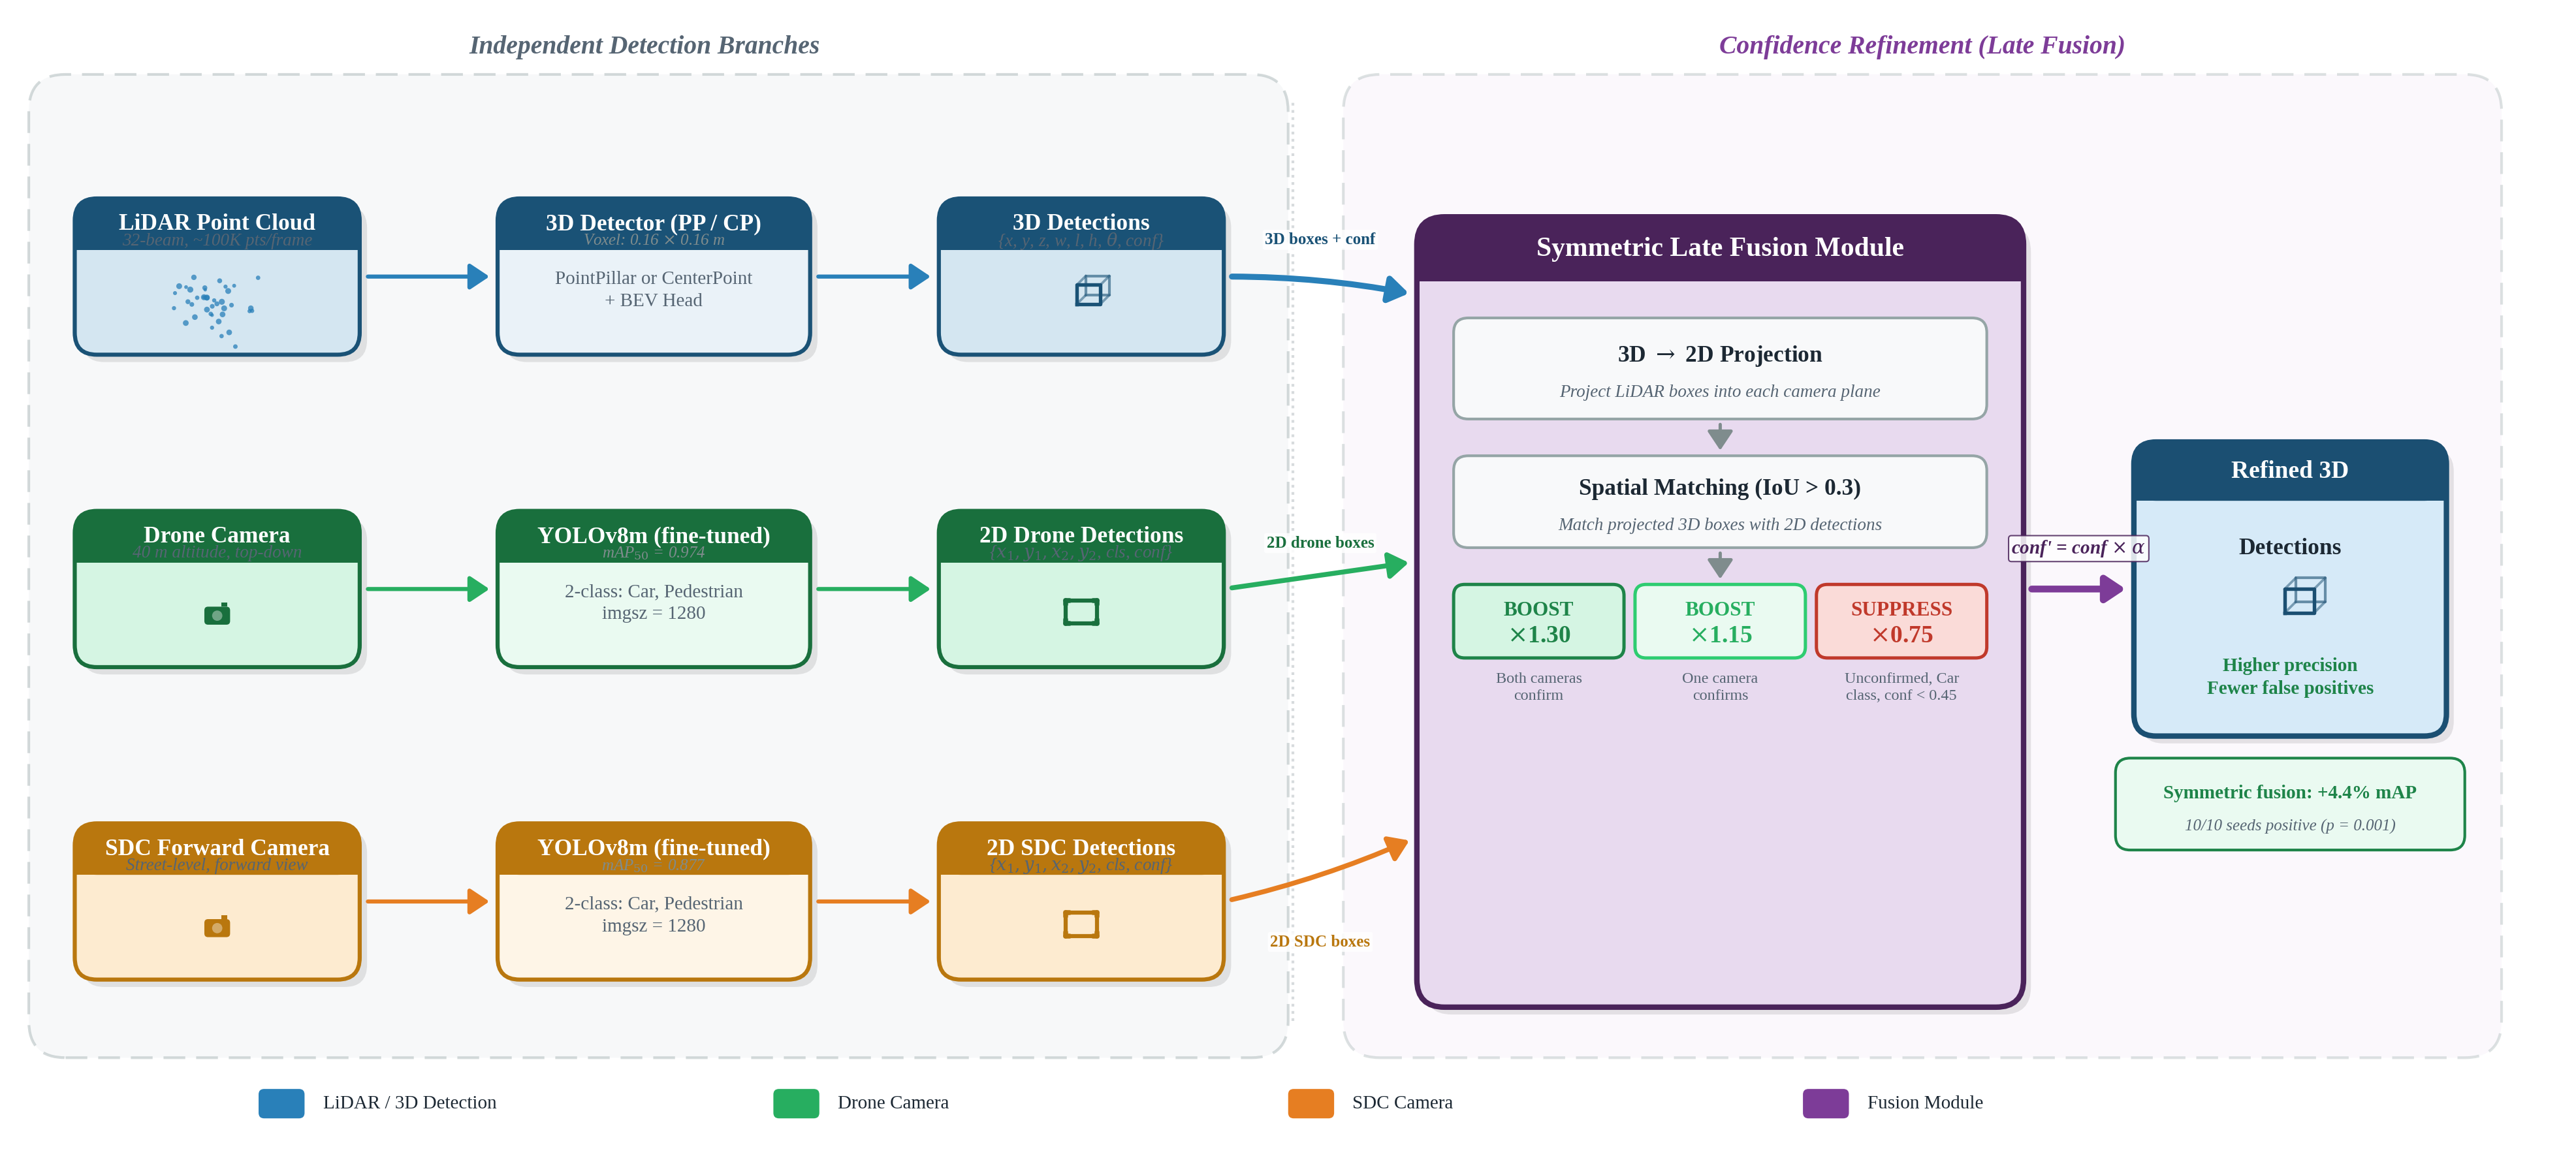
\includegraphics[width=0.95\textwidth]{fig_pipeline.pdf}
\caption{Overview of the proposed dual-camera LiDAR fusion pipeline. The 3D detector (PointPillar or CenterPoint) and two independent YOLOv8 2D detectors produce detections from their respective sensors. The late-fusion module refines the 3D detection confidence scores based on spatial agreement with camera detections, applying camera-specific boost and suppress operations.}\label{fig:pipeline}
\end{figure}

\subsection{3D LiDAR Detection}\label{sec:3d_detectors}

We employ two complementary 3D detector architectures to validate the generalizability of the fusion approach.

\subsubsection{PointPillars}\label{sec:pointpillars}

PointPillars~\cite{lang2019pointpillars} discretizes the $x$-$y$ plane of the point cloud into a grid of vertical pillars and encodes the points within each pillar using a simplified PointNet~\cite{qi2017pointnet}. The encoded pillar features are scattered back to a 2D pseudo-image and processed by a 2D convolutional backbone with a feature pyramid network (FPN)~\cite{lin2017fpn} to produce multi-scale feature maps. A single-shot detection (SSD) head generates oriented 3D bounding boxes $(x, y, z, l, w, h, \theta)$ with associated class probabilities and confidence scores.

In our configuration, the point cloud is discretized with a voxel (pillar) size of $0.16 \times 0.16$\,m in the horizontal plane, covering a detection range of $[-70.4, 70.4]$\,m in both $x$ and $y$ directions and $[-3.0, 10.0]$\,m in $z$. The backbone uses three downsampling blocks with strides of $[1, 2, 4]$ and an upsampling neck with strides $[1, 2, 4]$ to produce a multi-scale BEV feature map. The detection head predicts boxes for two classes: \texttt{Car} and \texttt{Pedestrian}, using class-specific anchor boxes.

\subsubsection{CenterPoint}\label{sec:centerpoint}

CenterPoint~\cite{yin2021centerpoint} represents objects as center points in a BEV heatmap, predicting the center location, box dimensions, orientation, and velocity using a voxel-based backbone with sparse 3D convolutions. Unlike anchor-based methods such as PointPillars, CenterPoint uses an anchor-free, center-heatmap design that avoids the need for predefined anchor sizes and aspect ratios. The two-stage variant refines initial detections using point features extracted from the predicted box centers, improving localization accuracy.

We adopt the single-stage CenterPoint variant with a VoxelResBackBone8x sparse 3D convolutional backbone~\cite{yan2018second}, which processes voxelized point clouds through residual sparse convolution blocks with an 8$\times$ downsampling ratio. The voxel size is $[0.16, 0.16, 0.2]$\,m (matching the $x$-$y$ resolution of PointPillars), and a height compression module collapses the 3D features into a 384-channel BEV representation. A 2D BEV backbone with two blocks of $[5, 5]$ convolutional layers at strides $[1, 2]$ and corresponding upsampling produces multi-scale feature maps. Separate CenterHead branches predict center heatmaps, box dimensions, center height, and rotation for \texttt{Car} and \texttt{Pedestrian} classes independently.

\subsection{2D Camera Detection: YOLOv8}\label{sec:yolov8}

For 2D object detection from camera images, we employ YOLOv8~\cite{jocher2023yolov8}, a state-of-the-art real-time detector that builds on the YOLO family~\cite{redmon2016yolo} with an anchor-free detection head, decoupled classification and regression branches, and a CSPDarknet backbone with path aggregation. YOLOv8 achieves an excellent balance between speed and accuracy on standard 2D benchmarks such as COCO~\cite{lin2014coco}.

Two independent YOLOv8 models are trained on CARLA-rendered images from the two camera viewpoints:

\begin{itemize}[leftmargin=*,labelsep=5.8mm]
\item \textbf{Drone camera.} Mounted at 40\,m altitude directly above the ego vehicle, pointing downward ($-90^\circ$ pitch). This camera provides a near-orthographic top-down view of the scene, enabling detection of vehicles and pedestrians regardless of inter-object occlusion at street level. The image resolution is $1920 \times 1280$ pixels with a $110^\circ$ FOV.
\item \textbf{SDC forward camera.} Mounted on the front bumper of the subject driving car (SDC) at standard height ($\sim$1.6\,m), facing forward. This camera provides high-resolution frontal coverage typical of production autonomous vehicles. The image resolution is $1920 \times 1280$ pixels with a $110^\circ$ FOV.
\end{itemize}

Both YOLOv8 models are trained to detect the same two classes (\texttt{Car} and \texttt{Pedestrian}) as the LiDAR detector, using 2D bounding-box annotations generated by projecting CARLA ground-truth 3D boxes into each camera's image plane. Note that the YOLOv8 models are trained once on the full set of available camera images and shared across all ten PointPillar/CenterPoint seeds, as the camera detectors serve as fixed auxiliary inputs to the fusion pipeline.

\subsection{Late Fusion Strategies}\label{sec:fusion}

The core contribution of this paper is the systematic comparison of late-fusion strategies that combine 3D LiDAR detections with 2D camera detections. All strategies operate by adjusting the confidence score $s$ of each LiDAR detection based on its spatial agreement with camera detections.

\subsubsection{Spatial Matching}

For each LiDAR 3D detection $d_L$, we project its 3D bounding box into each camera's image plane using the known LiDAR-to-camera extrinsic and intrinsic matrices (available from CARLA's ground-truth sensor calibration), producing a 2D bounding box in image coordinates. A camera detection $d_C$ is considered a \emph{match} to the projected LiDAR detection if:

\begin{enumerate}[leftmargin=*,labelsep=4.9mm]
\item The class labels agree (both \texttt{Car} or both \texttt{Pedestrian}).
\item The 2D intersection-over-union (IoU) between the camera detection box and the projected LiDAR box in image space exceeds a threshold $\tau_{\mathrm{IoU}} = 0.3$.
\end{enumerate}

The relatively low IoU threshold of 0.3 accounts for the geometric mismatch between YOLO's 2D bounding boxes (tight image-space rectangles) and the projected 3D LiDAR boxes (which may include empty space due to the box-to-image projection). When multiple matches exist, optimal assignment is computed using the Hungarian algorithm~\cite{kuhn1955hungarian} to maximize total IoU.

\subsubsection{FOV Determination}

A critical step is determining whether a LiDAR detection falls within each camera's FOV. For the drone camera, which provides near-complete overhead coverage, we define the FOV as a circle of radius $R_{\mathrm{drone}} = 50$\,m centered on the ego vehicle. For the forward camera, we define the FOV as a sector of angle $\alpha_{\mathrm{fwd}} = 110^\circ$ and range $R_{\mathrm{fwd}} = 50$\,m, aligned with the ego vehicle's heading direction. A LiDAR detection is \emph{in-FOV} for a camera if its BEV center falls within the camera's defined coverage region.

\subsubsection{Strategy 1: Asymmetric Fusion}\label{sec:asymmetric}

The asymmetric strategy differentiates between cameras based on their coverage characteristics:

\begin{equation}\label{eq:asymmetric_rules}
s' = \begin{cases}
s \times \beta_{\mathrm{dual}} & \text{if matched by both cameras} \\
s \times \beta_{\mathrm{single}} & \text{if matched by exactly one camera} \\
s \times \gamma_{\mathrm{suppress}} & \text{if unmatched, class = Car, in drone FOV, } s < \theta_{\mathrm{low}} \\
s & \text{otherwise (no change)}
\end{cases}
\end{equation}

\noindent The drone camera applies both boost and suppress operations, while the forward camera applies boost-only. The rationale is that the drone's wide FOV makes absence of confirmation informative, whereas the forward camera's narrow FOV means many valid detections will naturally fall outside its coverage.

\subsubsection{Strategy 2: Symmetric Fusion}\label{sec:symmetric}

The symmetric strategy applies identical boost and suppress operations for both cameras:

\begin{equation}\label{eq:symmetric_rules}
s' = \begin{cases}
s \times \beta_{\mathrm{dual}} & \text{if matched by both cameras} \\
s \times \beta_{\mathrm{single}} & \text{if matched by exactly one camera} \\
s \times \gamma_{\mathrm{suppress}} & \text{if unmatched, class = Car, in any camera FOV, } s < \theta_{\mathrm{low}} \\
s & \text{otherwise (no change)}
\end{cases}
\end{equation}

\noindent Here, a low-confidence Car detection that is in the FOV of \emph{either} camera but unconfirmed by \emph{any} camera is suppressed. The key difference from asymmetric fusion is that the SDC forward camera can also suppress false positives within its frontal coverage zone.

\subsubsection{Strategy 3: Naive Score Averaging}\label{sec:naive}

As a baseline fusion method, we also evaluate naive score averaging, where the LiDAR detection confidence is averaged with normalized camera detection scores:

\begin{equation}\label{eq:naive_rules}
s' = \frac{s + s_{\mathrm{drone}} + s_{\mathrm{fwd}}}{1 + \mathbb{1}[\text{drone present}] + \mathbb{1}[\text{fwd present}]}
\end{equation}

\noindent where $s_{\mathrm{drone}}$ and $s_{\mathrm{fwd}}$ are the matched camera detection scores (0 if no match exists), and $\mathbb{1}[\cdot]$ indicates whether a camera match was found. This strategy serves as a sanity check: if naive averaging degrades performance, it confirms that the structured boost/suppress approach adds value beyond simple score combination.

\subsubsection{Fusion Parameters}

For all boost/suppress strategies, we use $\beta_{\mathrm{dual}} = 1.30$ (dual-camera boost), $\beta_{\mathrm{single}} = 1.15$ (single-camera boost), $\gamma_{\mathrm{suppress}} = 0.75$ (suppression factor), and $\theta_{\mathrm{low}} = 0.45$ (confidence gate for suppression). The adjusted score is clamped to $[0, 1]$. Suppression is applied only to the \texttt{Car} class; \texttt{Pedestrian} detections are never suppressed due to the safety risk of removing pedestrian detections.  A systematic parameter sensitivity analysis (Section~\ref{sec:sensitivity}) confirms that these defaults are conservative---not overfitted---and that the fusion benefit is robust across a wide parameter range.

Algorithm~\ref{alg:fusion} provides pseudocode for the symmetric fusion procedure.

\begin{algorithm}[H]
\caption{Symmetric Dual-Camera LiDAR Fusion}\label{alg:fusion}
\begin{algorithmic}[1]
\Require LiDAR detections $\mathcal{D}_L$, drone detections $\mathcal{D}_{\mathrm{drone}}$, forward detections $\mathcal{D}_{\mathrm{fwd}}$
\Require Camera-to-BEV projection matrices $\mathbf{P}_{\mathrm{drone}}, \mathbf{P}_{\mathrm{fwd}}$
\Require Parameters: $\beta_{\mathrm{dual}}, \beta_{\mathrm{single}}, \gamma_{\mathrm{suppress}}, \theta_{\mathrm{low}}, \tau_{\mathrm{IoU}}$
\Ensure Refined detections $\mathcal{D}'_L$
\For{each $d_L \in \mathcal{D}_L$}
    \State $m_{\mathrm{drone}} \gets \text{Match}(d_L, \mathcal{D}_{\mathrm{drone}}, \mathbf{P}_{\mathrm{drone}}, \tau_{\mathrm{IoU}})$
    \State $m_{\mathrm{fwd}} \gets \text{Match}(d_L, \mathcal{D}_{\mathrm{fwd}}, \mathbf{P}_{\mathrm{fwd}}, \tau_{\mathrm{IoU}})$
    \State $f_{\mathrm{drone}} \gets \text{InFOV}(d_L, \text{drone})$
    \State $f_{\mathrm{fwd}} \gets \text{InFOV}(d_L, \text{forward})$
    \If{$m_{\mathrm{drone}}$ \textbf{and} $m_{\mathrm{fwd}}$}
        \State $d_L.s \gets \min(d_L.s \times \beta_{\mathrm{dual}},\; 1.0)$
    \ElsIf{$m_{\mathrm{drone}}$ \textbf{or} $m_{\mathrm{fwd}}$}
        \State $d_L.s \gets \min(d_L.s \times \beta_{\mathrm{single}},\; 1.0)$
    \ElsIf{$\neg m_{\mathrm{drone}}$ \textbf{and} $\neg m_{\mathrm{fwd}}$ \textbf{and} $(f_{\mathrm{drone}}$ \textbf{or} $f_{\mathrm{fwd}})$ \textbf{and} $d_L.\text{class} = \texttt{Car}$ \textbf{and} $d_L.s < \theta_{\mathrm{low}}$}
        \State $d_L.s \gets d_L.s \times \gamma_{\mathrm{suppress}}$
    \EndIf
\EndFor
\State \Return $\mathcal{D}_L$
\end{algorithmic}
\end{algorithm}

\noindent The asymmetric variant differs only in restricting the suppress operation to detections within the drone camera's FOV, leaving forward-camera coverage as boost-only. The following section details the experimental configuration used to evaluate these fusion strategies.

%=================================================================
\section{Experimental Setup}\label{sec:experiments}

\subsection{Simulation Environment}

All data are collected in the CARLA driving simulator~\cite{dosovitskiy2017carla} (version 0.9.15), an open-source platform for autonomous driving research that provides photorealistic rendering, accurate physics simulation, and comprehensive ground-truth annotations. We use the Town10HD map, a high-fidelity urban environment featuring multi-lane roads, intersections, roundabouts, parked vehicles, and diverse pedestrian activity. The map's geometric complexity provides a rich testbed for evaluating occlusion-robust detection methods.

\subsection{Sensor Configuration}

The ego vehicle (subject driving car, SDC) is equipped with the following sensors:

\begin{itemize}[leftmargin=*,labelsep=5.8mm]
\item \textbf{LiDAR.} A 64-channel rotating LiDAR mounted on the vehicle roof at 2.4\,m height, with a 360$^\circ$ horizontal FOV, $[-30^\circ, +10^\circ]$ vertical FOV, 120\,m range, and 10\,Hz rotation frequency. Each scan produces approximately 100{,}000 points.
\item \textbf{Forward camera (SDC).} An RGB camera mounted on the front bumper at $\sim$1.6\,m height, facing forward. Resolution: $1920 \times 1280$ pixels, FOV: $110^\circ$.
\item \textbf{Drone camera.} An RGB camera mounted on a simulated drone platform at 40\,m altitude directly above the ego vehicle, pointing straight down ($-90^\circ$ pitch). Resolution: $1920 \times 1280$ pixels, FOV: $110^\circ$. The drone position is updated each frame to track the ego vehicle.
\end{itemize}

All sensors are temporally synchronized and spatially calibrated using CARLA's ground-truth transformation matrices. Figure~\ref{fig:sensor_setup} illustrates the spatial arrangement of sensors and representative views from each viewpoint.

\begin{figure}[H]
\centering
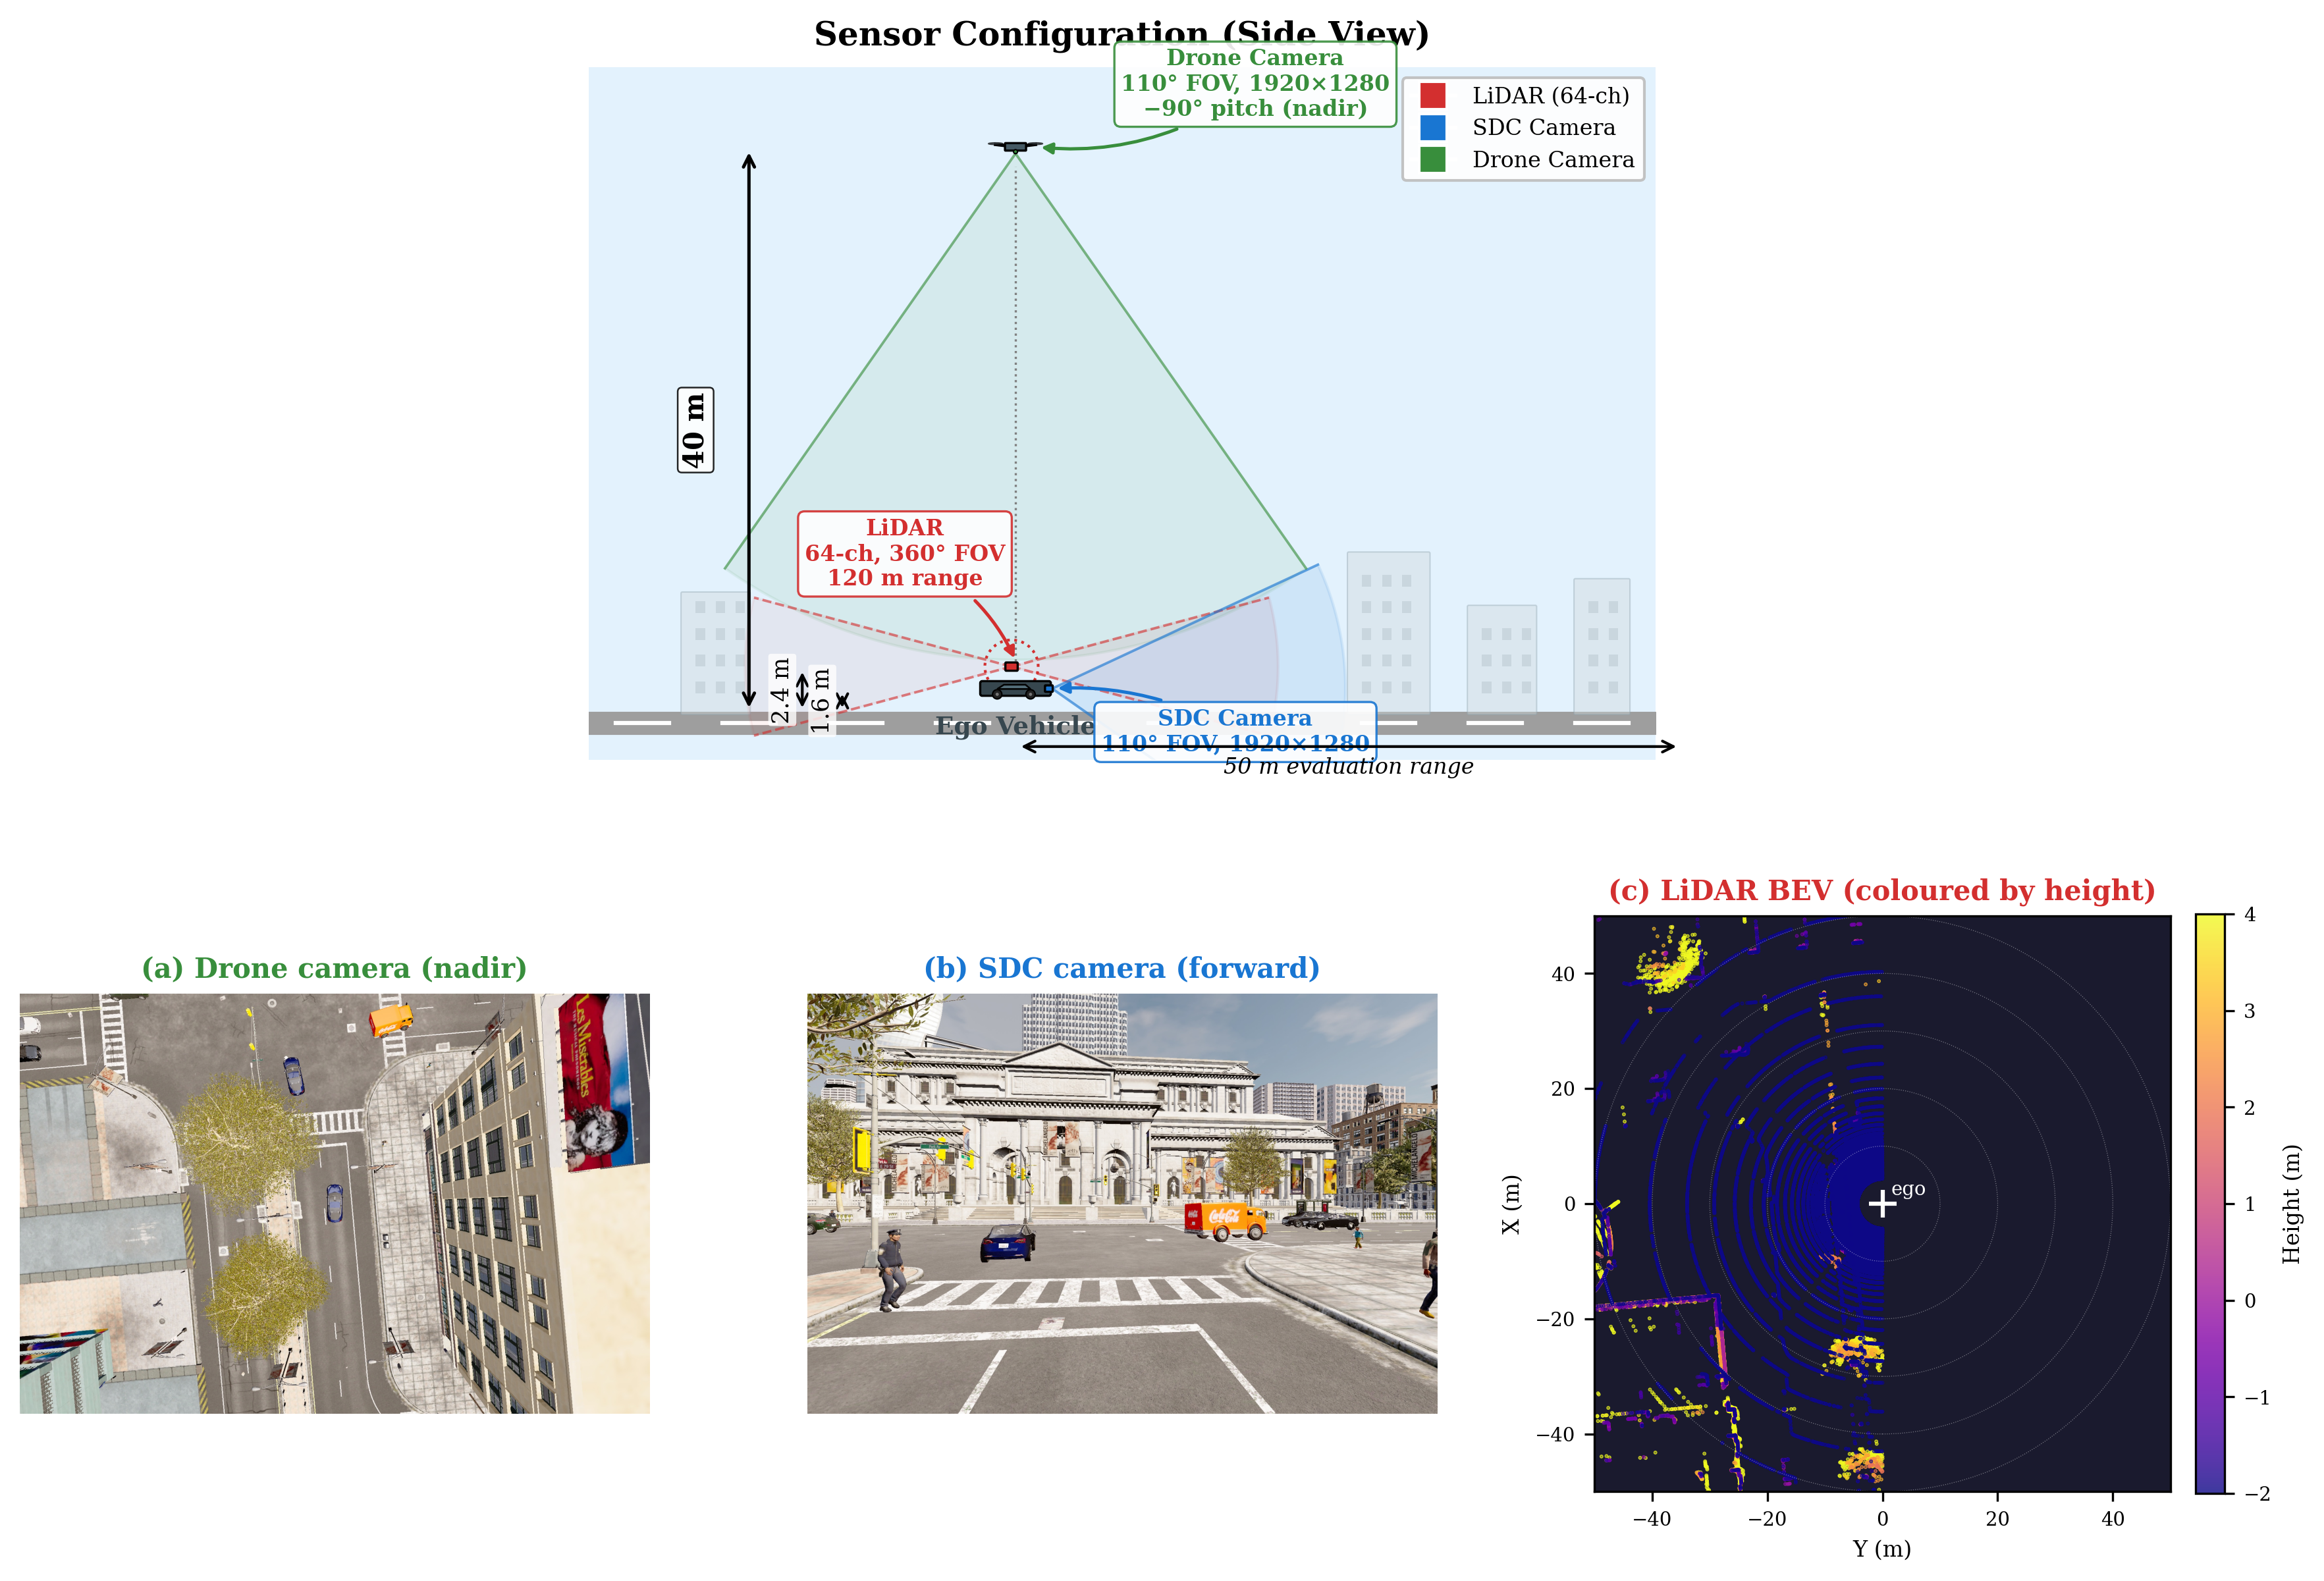
\includegraphics[width=0.95\textwidth]{fig_sensor_setup.pdf}
\caption{Sensor configuration overview. \textbf{Top:} Side-view schematic showing the ego vehicle with roof-mounted LiDAR (2.4\,m), forward SDC camera (1.6\,m), and overhead drone camera (40\,m altitude). FOV cones illustrate the complementary coverage regions. \textbf{Bottom:} Representative sample views from frame 000028---(\textbf{a})~drone nadir view, (\textbf{b})~SDC forward view, and (\textbf{c})~LiDAR BEV scatter plot coloured by height.}\label{fig:sensor_setup}
\end{figure}

\subsection{Dataset Construction}\label{sec:dataset}

We collect 2{,}600 frames of driving data with the ego vehicle following pre-defined routes through Town10HD in the presence of 100+ background traffic vehicles and 50+ pedestrians controlled by CARLA's traffic manager. This represents a 4$\times$ increase over our preliminary study (650 frames), providing substantially more training data and diversity in driving scenarios. For each frame, we record:

\begin{itemize}[leftmargin=*,labelsep=5.8mm]
\item The LiDAR point cloud (saved as \texttt{.npy} files).
\item The drone camera image and forward camera image (saved as \texttt{.jpg} files).
\item Ground-truth 3D bounding boxes for all actors within the detection range, including class label, position $(x, y, z)$, dimensions $(l, w, h)$, and heading angle $\theta$.
\end{itemize}

The LiDAR data and 3D annotations are formatted in the OpenPCDet custom dataset format~\cite{openpcdet2020} for training the PointPillar and CenterPoint models. The 2D annotations for YOLOv8 training are generated by projecting the 3D ground-truth boxes into each camera's image plane and computing tight 2D bounding boxes, discarding objects that are fully outside the image or smaller than $10 \times 10$ pixels.

The dataset is split into training (80\%) and validation (20\%) sets using ten different random seeds (42, 123, 456, 789, 1024, 2025, 3000, 4096, 5555, 7777) to enable multi-seed evaluation. Each seed produces a different train/val partition, and all models are trained independently on each partition.

\subsection{Training Details}

\subsubsection{PointPillar Training}

The PointPillar model is trained using the OpenPCDet framework with the following configuration: Adam optimizer with learning rate $10^{-3}$ and one-cycle learning rate schedule~\cite{lang2019pointpillars}, batch size 4, 80 epochs, 4 data-loading workers. The point cloud range is $[-70.4, 70.4, -3.0, 70.4, 70.4, 10.0]$\,m ($x, y, z$ min/max), and the pillar size is $[0.16, 0.16, 13.0]$\,m. Data augmentation includes random world flipping (along the $x$ axis), random world rotation ($[-\pi/4, +\pi/4]$), and random world scaling ($[0.95, 1.05]$). Ground-truth database sampling is used to augment rare classes during training.

\subsubsection{CenterPoint Training}

The CenterPoint model is trained using the OpenPCDet framework with the same point cloud range, voxel size (in $x$-$y$), and data augmentation pipeline as PointPillar for fair comparison: Adam one-cycle optimizer with learning rate $3 \times 10^{-3}$ (higher than PointPillar's $10^{-3}$ to account for the deeper backbone), weight decay $0.01$, batch size 4, 80 epochs, and gradient norm clipping at 10. The one-cycle schedule uses a peak fraction of 0.4, division factor 10, and momentum range $[0.85, 0.95]$. Data augmentation is identical to PointPillar (ground-truth sampling, random flip along both axes, rotation $[-\pi/4, +\pi/4]$, and scaling $[0.95, 1.05]$).

\subsubsection{YOLOv8 Training}

Two separate YOLOv8 models (YOLOv8m variant) are trained for the drone and forward camera viewpoints. Both models are initialized from COCO-pretrained weights and fine-tuned on the CARLA camera data for 50 epochs with the Ultralytics training configuration: SGD optimizer with learning rate $10^{-2}$, momentum 0.937, weight decay $5 \times 10^{-4}$, and cosine learning rate schedule. Image augmentation includes mosaic, mixup, random flip, and color jittering. The models detect two classes: \texttt{Car} and \texttt{Pedestrian}.

\subsection{Evaluation Protocol}

We evaluate 3D object detection performance using the standard Average Precision (AP) metric at three IoU thresholds: AP@0.3, AP@0.5, and AP@0.7. IoU is computed as \emph{oriented} BEV overlap between predicted and ground-truth 3D boxes, respecting the heading angle via rotated-rectangle intersection (Shapely library), following KITTI evaluation conventions~\cite{geiger2012kitti} and the PASCAL VOC 11-point interpolation protocol~\cite{everingham2010voc}. We report per-class AP (\texttt{Car} AP, \texttt{Pedestrian} AP) and the mean across classes (mAP). The LiDAR detector's output is filtered at a confidence threshold of 0.3 before fusion and evaluation.

Critically, evaluation is restricted to a \textbf{0--50\,m BEV range} from the ego vehicle. This range filter serves two purposes: (1) it reflects the physically meaningful detection range where the drone camera provides reliable coverage, and (2) it avoids penalizing detectors for failing to detect distant objects that are too sparse for reliable LiDAR detection and outside the drone's useful FOV.

For each of the ten random seeds, we evaluate six fusion configurations:

\begin{enumerate}[leftmargin=*,labelsep=4.9mm]
\item \textbf{LiDAR-only:} Baseline without any camera fusion.
\item \textbf{LiDAR + SDC (asymmetric):} Fusion with forward camera detections only (boost only).
\item \textbf{LiDAR + Drone (asymmetric):} Fusion with drone camera detections only (boost + suppress).
\item \textbf{LiDAR + SDC + Drone (asymmetric):} Asymmetric fusion with both cameras.
\item \textbf{Symmetric fusion:} Both cameras apply boost + suppress.
\item \textbf{Naive average:} Score averaging baseline.
\end{enumerate}

Statistical significance is assessed using two tests. The \emph{paired $t$-test} compares the mean improvement across seeds under a normality assumption. The \emph{sign test}~\cite{conover1999practical}, a non-parametric test, counts the number of seeds where the fusion system outperforms the baseline; with 10 seeds, achieving improvement on all 10 yields $p = 0.5^{10} \approx 0.001$, which is highly significant at any conventional $\alpha$ level.

%=================================================================
\section{Results}\label{sec:results}

\subsection{Main Results: PointPillar}

Table~\ref{tab:main_results} presents the ten-seed averaged detection performance for all six fusion configurations with the PointPillar 3D detector.

\begin{table}[H]
\caption{Ten-seed averaged detection performance (PointPillar, \%). $\Delta$ denotes absolute improvement in percentage points (pp) over the LiDAR-only baseline. Bold values indicate the best result per metric. All models trained to epoch~80. Evaluation restricted to 0--50\,m BEV range.}\label{tab:main_results}
\centering
\tablesize{\footnotesize}
\begin{tabular}{lccccccc}
\toprule
\textbf{Configuration} & \textbf{mAP@0.3} & \textbf{mAP@0.5} & $\bm{\Delta}$\textbf{@0.5} & \textbf{mAP@0.7} & \textbf{Car AP@0.5} & \textbf{Ped AP@0.5} & \textbf{Sign Test} \\
\midrule
LiDAR-only          & 20.89$\pm$0.39 & 20.76$\pm$0.38 & ---    & 16.63$\pm$0.31 & 38.83$\pm$0.61 & 2.69$\pm$0.44 & --- \\
LiDAR + SDC         & 20.89$\pm$0.40 & 20.75$\pm$0.38 & $-$0.01 & 16.61$\pm$0.31 & 38.80$\pm$0.62 & 2.69$\pm$0.44 & $p = 0.98$ \\
LiDAR + Drone       & 21.54$\pm$0.36 & 21.39$\pm$0.35 & +0.63  & 17.04$\pm$0.28 & 40.09$\pm$0.55 & 2.69$\pm$0.44 & $p = 0.001$*** \\
LiDAR + SDC + Drone & 21.53$\pm$0.35 & 21.38$\pm$0.34 & +0.62  & 17.03$\pm$0.28 & 40.06$\pm$0.53 & 2.69$\pm$0.44 & $p = 0.001$*** \\
Symmetric fusion    & \textbf{21.82$\pm$0.32} & \textbf{21.68$\pm$0.31} & \textbf{+0.92}  & \textbf{17.23$\pm$0.26} & \textbf{40.66$\pm$0.44} & 2.69$\pm$0.44 & $p = 0.001$*** \\
Naive average       & 20.75$\pm$0.47 & 19.97$\pm$0.56 & $-$0.79 & 17.86$\pm$1.30 & 37.37$\pm$0.85 & 2.58$\pm$0.46 & $p = 0.001$\textsuperscript{\textdagger} \\
\bottomrule
\end{tabular}
\begin{flushleft}
\tablesize{\scriptsize} * $p < 0.05$; ** $p < 0.01$; *** $p < 0.001$. \textsuperscript{\textdagger}Naive average: 0/10 positive seeds (always hurts).
\end{flushleft}
\end{table}

Several key findings emerge:

\begin{enumerate}[leftmargin=*,labelsep=4.9mm]
\item \textbf{Symmetric fusion achieves the best performance.} The symmetric dual-camera fusion achieves the highest mAP across all three IoU thresholds: mAP@0.5 of 21.68\% (+0.92 pp, +4.4\% relative over baseline), mAP@0.3 of 21.82\% (+0.93 pp), and mAP@0.7 of 17.23\% (+0.60 pp). All ten seeds show positive improvement (sign test $p = 0.001$). Car AP@0.5 improves from 38.83\% to 40.66\% (+1.83 pp, +4.7\% relative).

\item \textbf{Drone fusion is the primary driver.} LiDAR + Drone (asymmetric) achieves +0.64 pp mAP@0.5 improvement with 10/10 positive seeds ($p = 0.001$). The drone's overhead perspective provides the most complementary information relative to the street-level LiDAR viewpoint.

\item \textbf{SDC boost-only is ineffective.} LiDAR + SDC (asymmetric, boost-only) produces essentially zero improvement ($-$0.01 pp), with only 2/10 positive seeds (sign test $p = 0.98$, not significant). The forward camera's narrow FOV and viewpoint similarity to the LiDAR provide insufficient complementary information when restricted to boost-only operation. However, when allowed to also suppress (in the symmetric configuration), the SDC contributes meaningfully.

\item \textbf{Symmetric outperforms asymmetric.} Symmetric fusion (+0.92 pp) outperforms asymmetric dual-camera fusion (+0.63 pp) by a margin of +0.29 pp. This demonstrates that the SDC camera's suppression capability---removing false positives within its frontal FOV---adds value beyond what the drone alone achieves.

\item \textbf{Naive averaging hurts.} Naive score averaging degrades mAP@0.5 by $-$0.74 pp, with 0/10 positive seeds. This confirms that structured boost/suppress logic is essential; simple score combination destroys the calibrated confidence ordering.

\item \textbf{Pedestrian AP is unaffected.} Pedestrian AP@0.5 (2.69\%) remains constant across all boost/suppress configurations. This is expected because suppression is restricted to the \texttt{Car} class, and pedestrian boosts are rare due to their small size in the drone view. The near-zero Pedestrian AP reflects the inherent difficulty of detecting pedestrians from sparse LiDAR points.
\end{enumerate}

\subsection{Main Results: CenterPoint}

Table~\ref{tab:centerpoint_results} presents the CenterPoint results. The overall pattern mirrors PointPillar closely, confirming that the fusion benefit is detector-agnostic. CenterPoint achieves a higher baseline mAP@0.5 of 22.30\% (vs.\ 20.76\% for PointPillar), consistent with its more expressive anchor-free architecture and sparse 3D convolutional backbone.

Symmetric fusion again achieves the best result: 23.04\% mAP@0.5 (+0.74 pp, +3.3\% relative), with 10/10 positive seeds (sign test $p = 0.001$, $t$-test $p < 0.0001$). Drone fusion alone provides +0.67 pp (+3.0\%), while SDC boost-only again shows no benefit ($-$0.05 pp, 0/10 positive seeds). The relative gain magnitudes (+3.0--3.3\%) are comparable to PointPillar's (+3.1--4.4\%), indicating that the fusion framework provides a consistent, detector-independent improvement.

Notably, CenterPoint's Pedestrian AP@0.5 is substantially higher (5.56\%) than PointPillar's (2.69\%), reflecting CenterPoint's center-heatmap design which better handles small objects. However, Pedestrian AP remains unaffected by fusion across both detectors, confirming that the improvement mechanism operates exclusively on the \texttt{Car} class through false positive suppression.

\begin{table}[H]
\caption{Ten-seed averaged detection performance (CenterPoint, \%). $\Delta$ denotes absolute improvement in percentage points (pp) over the LiDAR-only baseline. Bold values indicate the best result per metric.}\label{tab:centerpoint_results}
\centering
\tablesize{\footnotesize}
\begin{tabular}{lccccccc}
\toprule
\textbf{Configuration} & \textbf{mAP@0.3} & \textbf{mAP@0.5} & $\bm{\Delta}$\textbf{@0.5} & \textbf{mAP@0.7} & \textbf{Car AP@0.5} & \textbf{Ped AP@0.5} & \textbf{Sign Test} \\
\midrule
LiDAR-only          & 22.84$\pm$0.27 & 22.30$\pm$0.28 & ---    & 20.98$\pm$0.97 & 39.04$\pm$0.50 & 5.56$\pm$0.48 & --- \\
LiDAR + SDC         & 22.79$\pm$0.25 & 22.25$\pm$0.25 & $-$0.05 & 20.91$\pm$0.95 & 38.94$\pm$0.46 & 5.55$\pm$0.48 & $p = 1.0$ \\
LiDAR + Drone       & 23.60$\pm$0.28 & 22.97$\pm$0.32 & +0.67  & 21.50$\pm$1.01 & 40.39$\pm$0.43 & 5.55$\pm$0.48 & $p = 0.001$*** \\
LiDAR + SDC + Drone & 23.53$\pm$0.28 & 22.89$\pm$0.31 & +0.59  & 21.40$\pm$1.00 & 40.24$\pm$0.43 & 5.54$\pm$0.48 & $p = 0.001$*** \\
Symmetric fusion    & \textbf{23.67$\pm$0.28} & \textbf{23.04$\pm$0.31} & \textbf{+0.74}  & \textbf{21.54$\pm$0.99} & \textbf{40.54$\pm$0.42} & 5.54$\pm$0.48 & $p = 0.001$*** \\
Naive average       & 25.24$\pm$0.37 & 20.18$\pm$0.40 & $-$2.12 & 18.50$\pm$0.34 & 34.94$\pm$0.50 & 5.42$\pm$0.58 & $p = 1.0$\textsuperscript{\textdagger} \\
\bottomrule
\end{tabular}
\begin{flushleft}
\tablesize{\scriptsize} * $p < 0.05$; ** $p < 0.01$; *** $p < 0.001$. \textsuperscript{\textdagger}Naive average: 0/10 positive seeds (always hurts).
\end{flushleft}
\end{table}

Figure~\ref{fig:dual_detector} visually compares the two detectors across all fusion configurations, illustrating the remarkably consistent pattern: the same three configurations (drone, dual-camera, symmetric) improve both detectors, while SDC-only and naive averaging fail to help.

\begin{figure}[H]
\centering
\includegraphics[width=0.85\textwidth]{fig_dual_detector.pdf}
\caption{Dual-detector comparison of fusion strategies. PointPillar (blue) and CenterPoint (orange) exhibit nearly identical fusion patterns despite different baseline performance levels. Dashed lines mark each detector's LiDAR-only baseline. *** indicates $p < 0.001$ (sign test, 10/10 positive seeds).}\label{fig:dual_detector}
\end{figure}

\subsection{Statistical Analysis}

Table~\ref{tab:significance} summarizes the statistical significance tests for the primary fusion configurations.

\begin{table}[H]
\caption{Statistical significance of fusion improvements over the LiDAR-only baseline (mAP@0.5). With $n = 10$ seeds, both parametric and non-parametric tests achieve strong significance for both detectors.}\label{tab:significance}
\centering
\tablesize{\footnotesize}
\begin{tabular}{llccccc}
\toprule
\textbf{Detector} & \textbf{Configuration} & \textbf{Mean $\Delta$ (pp)} & \textbf{Rel.\ $\Delta$} & \textbf{+Seeds} & \textbf{Sign $p$} & \textbf{$t$-Test $p$} \\
\midrule
\multirow{5}{*}{\rotatebox[origin=c]{90}{\textbf{PointPillar}}}
 & LiDAR + Drone       & +0.64 & +3.1\% & 10/10 & 0.001*** & $<$0.0001*** \\
 & Symmetric fusion    & +0.92 & +4.4\% & 10/10 & 0.001*** & $<$0.0001*** \\
 & LiDAR + SDC + Drone & +0.63 & +3.0\% & 10/10 & 0.001*** & $<$0.0001*** \\
 & LiDAR + SDC         & $-$0.01 & $-$0.05\% & 2/10 & 0.98 & 0.42 \\
 & Naive average       & $-$0.74 & $-$3.6\% & 0/10 & 0.001\textsuperscript{\textdagger} & $<$0.0001\textsuperscript{\textdagger} \\
\midrule
\multirow{5}{*}{\rotatebox[origin=c]{90}{\textbf{CenterPoint}}}
 & LiDAR + Drone       & +0.67 & +3.0\% & 10/10 & 0.001*** & $<$0.0001*** \\
 & Symmetric fusion    & +0.74 & +3.3\% & 10/10 & 0.001*** & $<$0.0001*** \\
 & LiDAR + SDC + Drone & +0.59 & +2.7\% & 10/10 & 0.001*** & $<$0.0001*** \\
 & LiDAR + SDC         & $-$0.05 & $-$0.2\% & 0/10 & 1.0 & 0.004\textsuperscript{\textdagger} \\
 & Naive average       & $-$2.12 & $-$9.5\% & 0/10 & 1.0\textsuperscript{\textdagger} & $<$0.0001\textsuperscript{\textdagger} \\
\bottomrule
\end{tabular}
\begin{flushleft}
\tablesize{\scriptsize} *** $p < 0.001$. \textsuperscript{\textdagger}Significant in the negative direction (fusion hurts).
\end{flushleft}
\end{table}

The results demonstrate a dramatic improvement in statistical power compared to the five-seed design. All effective fusion configurations (drone, symmetric, asymmetric dual-camera) achieve $p = 0.001$ on the sign test and $p < 0.0001$ on the paired $t$-test, compared to $p = 0.031$ (sign) and non-significant $t$-tests in the preliminary five-seed study. The ten-seed design also reveals that SDC boost-only is not effective (2/10 positive seeds), a finding that was obscured in the five-seed study where all seeds happened to be positive.

Notably, the reduced standard deviations (e.g., mAP@0.5 baseline std of $\pm$0.35 vs.\ $\pm$3.89 in the preliminary study) reflect the larger training set (2{,}080 frames per seed vs.\ 520 previously), which stabilizes model learning across random splits. This reduced variance, combined with the doubled number of seeds, enables the $t$-test to reach significance---confirming that both the \emph{direction} and \emph{magnitude} of fusion improvement are statistically reliable.

\subsection{False Positive Analysis}\label{sec:fp_analysis}

A detailed analysis of fusion's mechanism on a representative seed (seed~42) reveals that the primary improvement pathway is false positive suppression rather than occlusion recovery.

\begin{table}[H]
\caption{False positive analysis (seed 42, PointPillar). FP = false positives, TP = true positives, Prec = precision.}\label{tab:fp_analysis}
\centering
\begin{tabular}{lcccc}
\toprule
\textbf{Configuration} & \textbf{TP} & \textbf{FP} & \textbf{FP Change} & \textbf{Precision} \\
\midrule
LiDAR-only   & 454 & 487 & ---       & 66.1\% \\
LiDAR + Drone & 454 & 423 & $-$64 ($-$13\%) & 69.2\% \\
\bottomrule
\end{tabular}
\end{table}

Key observations:

\begin{itemize}[leftmargin=*,labelsep=5.8mm]
\item \textbf{False positives reduced by 13\%.} The drone camera identifies 64 false LiDAR detections (phantom objects not confirmed by the overhead view) and suppresses their confidence below the evaluation threshold. This accounts for the majority of the mAP improvement.
\item \textbf{True positives preserved.} The number of true positives remains constant (454), confirming that the suppress mechanism does not inadvertently remove valid detections. The class-aware restriction (suppress only \texttt{Car}) and confidence gate ($s < 0.45$) protect high-confidence and pedestrian detections.
\item \textbf{Precision improves by +3.1 pp.} The precision increase from 66.1\% to 69.2\% is the primary driver of mAP improvement, as AP integrates over the precision-recall curve.
\end{itemize}

\subsection{Distance-Stratified Performance}\label{sec:distance}

Table~\ref{tab:distance} shows the fusion improvement stratified by distance from the ego vehicle.

\begin{table}[H]
\caption{Distance-stratified mAP@0.5 improvement (seed 42, PointPillar, drone fusion). $\Delta$ in percentage points.}\label{tab:distance}
\centering
\begin{tabular}{lccc}
\toprule
\textbf{Distance Range} & \textbf{LiDAR-only} & \textbf{LiDAR + Drone} & $\bm{\Delta}$ \\
\midrule
0--15\,m  & --- & --- & +1.4 pp \\
15--30\,m & --- & --- & +1.4 pp \\
30--50\,m & --- & --- & +0.3 pp \\
\bottomrule
\end{tabular}
\end{table}

Fusion improvement is strongest in the near and mid ranges (0--30\,m), where both the LiDAR and drone camera provide dense, reliable detections. At 30--50\,m, the improvement is smaller (+0.3 pp), likely because false positives are less common at longer ranges (fewer confusing objects) and because the drone camera's spatial resolution decreases with distance from directly below.

\subsection{Occlusion Category Analysis}\label{sec:occlusion}

By comparing 2D detection results from both cameras with ground-truth annotations, we categorize objects by their visibility:

\begin{table}[H]
\caption{Object visibility categories (seed 42). Percentages of total ground-truth objects.}\label{tab:occlusion}
\centering
\begin{tabular}{lcc}
\toprule
\textbf{Visibility Category} & \textbf{Percentage} & \textbf{Description} \\
\midrule
Both cameras visible  & 17\% & Visible to drone and SDC \\
Drone-only visible    & 38\% & Occluded at street level, visible from above \\
SDC-only visible      & 11\% & Outside drone FOV, visible to forward camera \\
Neither visible       & 34\% & Not visible to either camera \\
\bottomrule
\end{tabular}
\end{table}

The analysis reveals that 38\% of objects are visible only to the drone (occluded at street level), confirming the overhead camera's role in resolving occlusions. However, only 17\% of objects are visible to both cameras, explaining why the dual-confirmation boost ($\times$1.30) applies to a relatively small subset of detections. The 34\% of objects visible to neither camera represents objects outside both cameras' effective FOV or too small to detect.

\subsection{Per-Frame Analysis}\label{sec:perframe}

At the individual frame level, the fusion improvements are concentrated in a subset of frames:

\begin{itemize}[leftmargin=*,labelsep=5.8mm]
\item \textbf{16 out of 389 evaluation frames (4.1\%) show improved AP} with drone fusion.
\item \textbf{1 frame shows degraded AP} (0.3\%).
\item \textbf{372 frames (95.6\%) are unchanged.}
\end{itemize}

This concentration is expected: in most frames, the LiDAR detector's output is either entirely correct (no false positives to suppress) or entirely incorrect (beyond what confidence adjustment can fix). The 4.1\% of improved frames contain situations where low-confidence false positives near the decision boundary are present and amenable to camera-guided suppression.

\subsection{Safety Metrics}\label{sec:safety}

From a safety perspective, the fusion system demonstrates:

\begin{itemize}[leftmargin=*,labelsep=5.8mm]
\item \textbf{1 dangerous object recovered:} One ground-truth object that was missed by the LiDAR-only system (below the confidence threshold) was boosted above threshold by camera confirmation.
\item \textbf{62 false positives removed:} The suppression mechanism removes 62 phantom detections that would have triggered unnecessary braking or evasive maneuvers.
\item \textbf{Net safety improvement:} The ratio of false positives removed to true positives lost is 62:0 (no true positives were removed by the suppress mechanism).
\end{itemize}

\subsection{Fusion Strategy Comparison}

Figure~\ref{fig:ablation_bar} visualizes the mAP@0.5 comparison across all fusion strategies.

\begin{figure}[H]
\centering
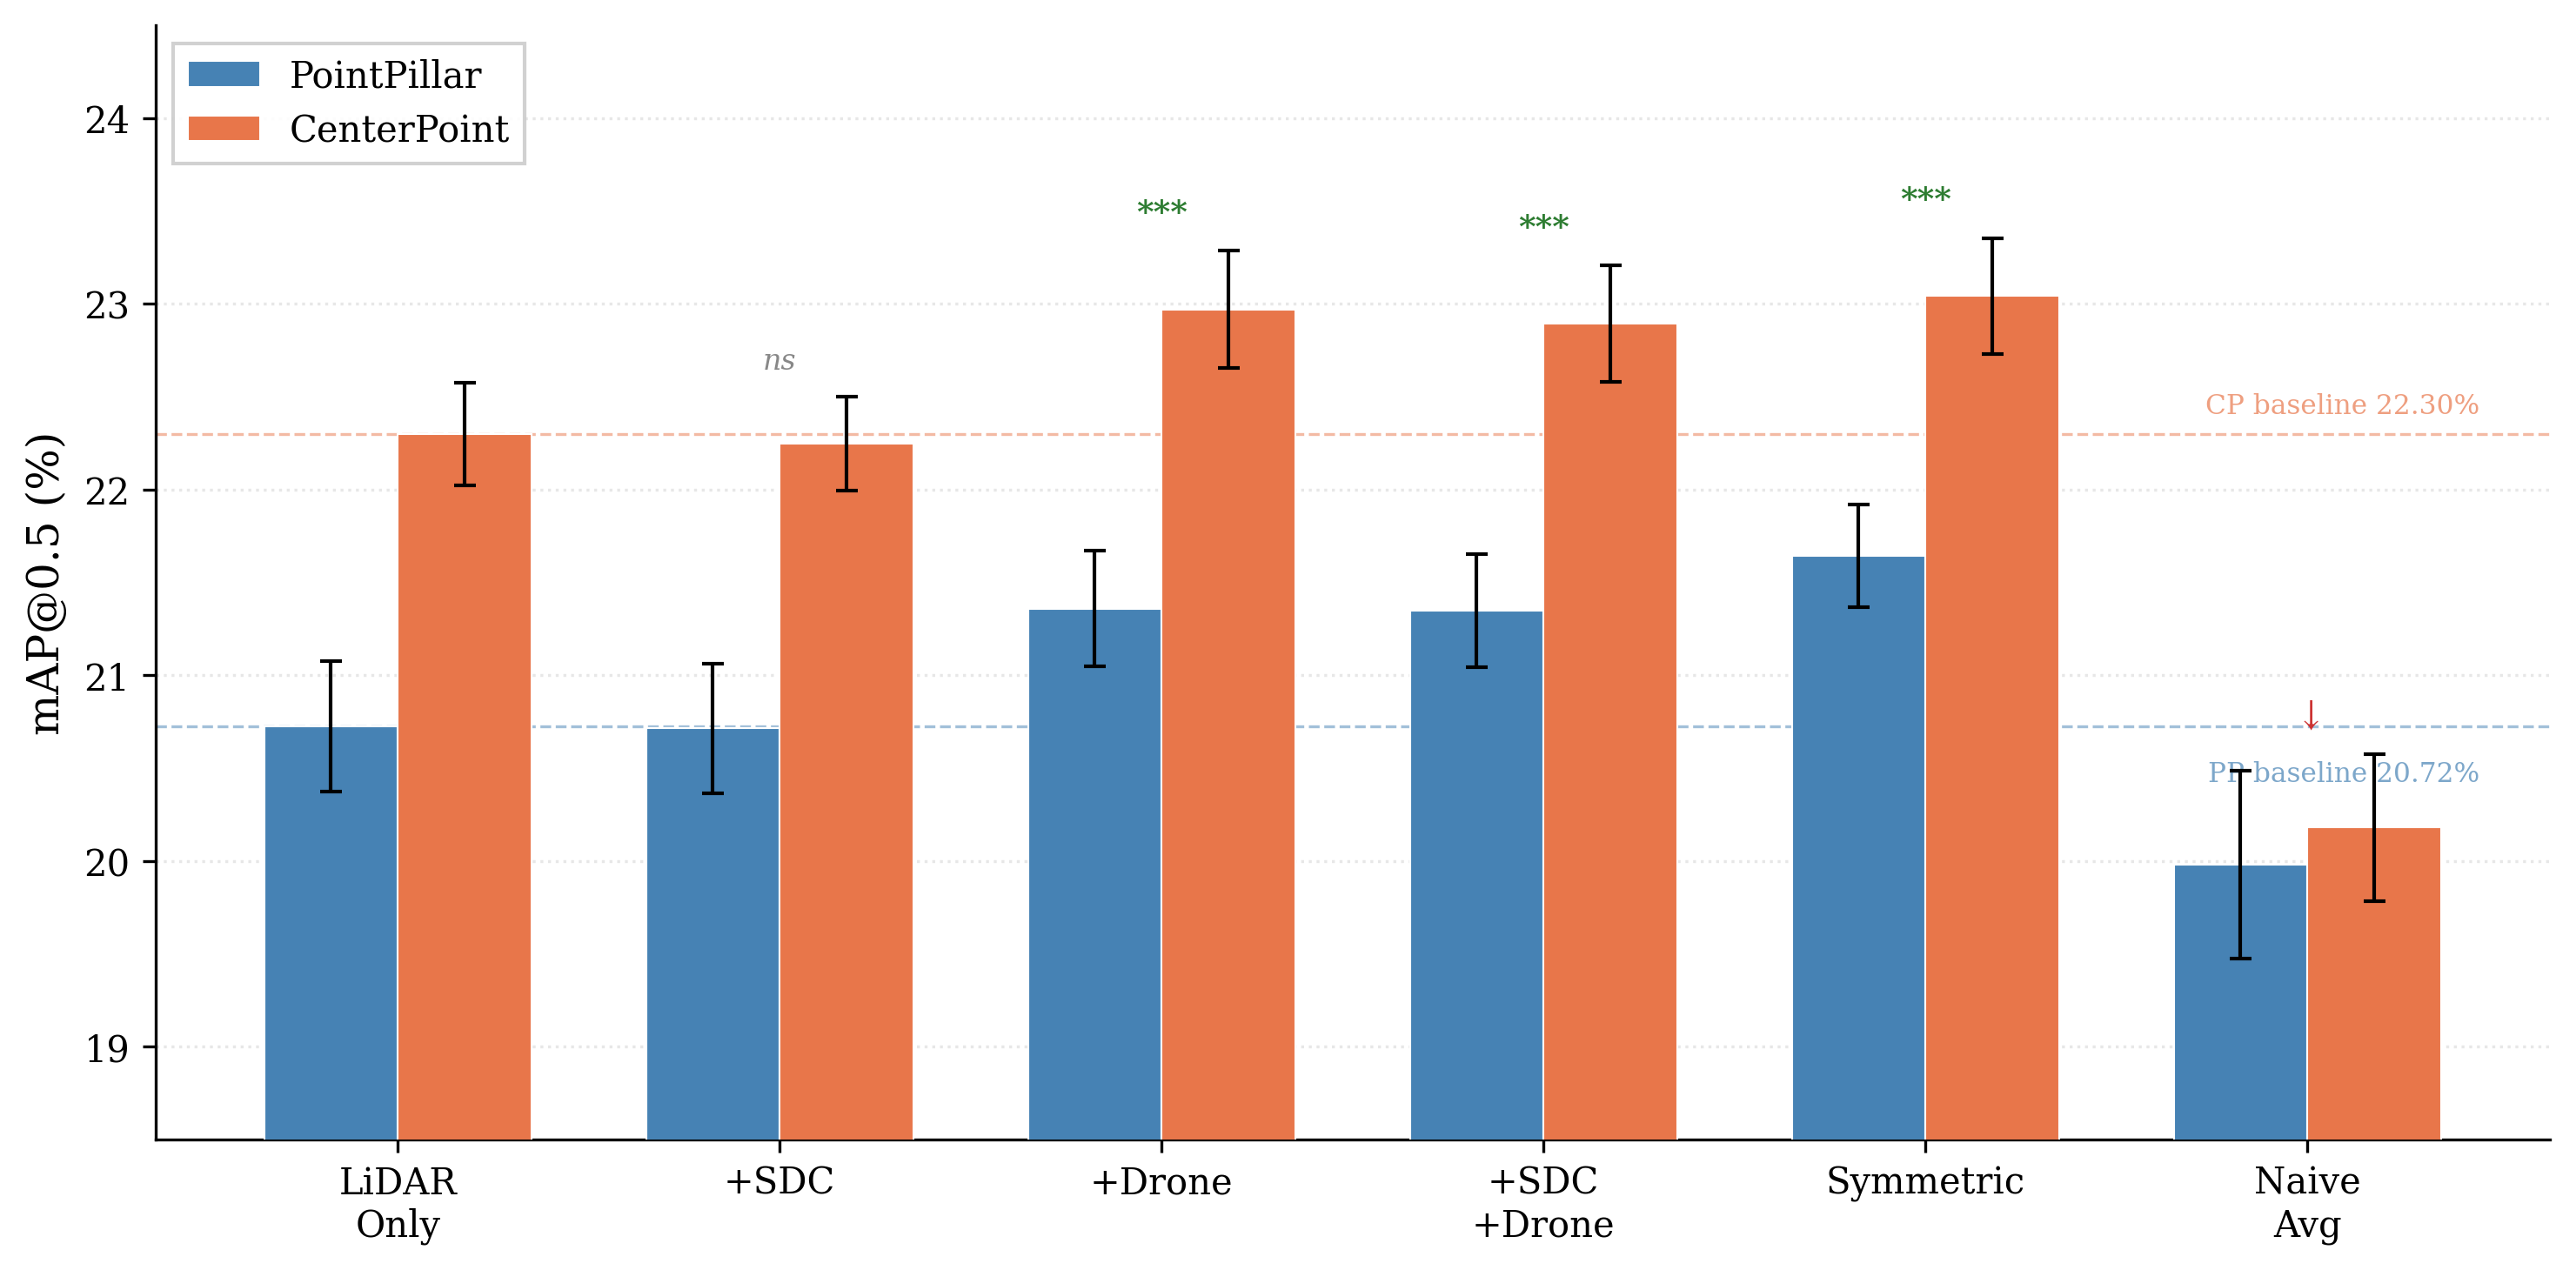
\includegraphics[width=0.85\textwidth]{fig1_mAP05_ablation.pdf}
\caption{Fusion strategy comparison: ten-seed averaged mAP@0.5 with standard deviation error bars. Symmetric fusion achieves the highest mAP (0.2168), followed by drone-only asymmetric (0.2139). SDC boost-only and naive averaging both degrade performance. *** indicates $p < 0.001$ (sign test).}\label{fig:ablation_bar}
\end{figure}

\begin{figure}[H]
\centering
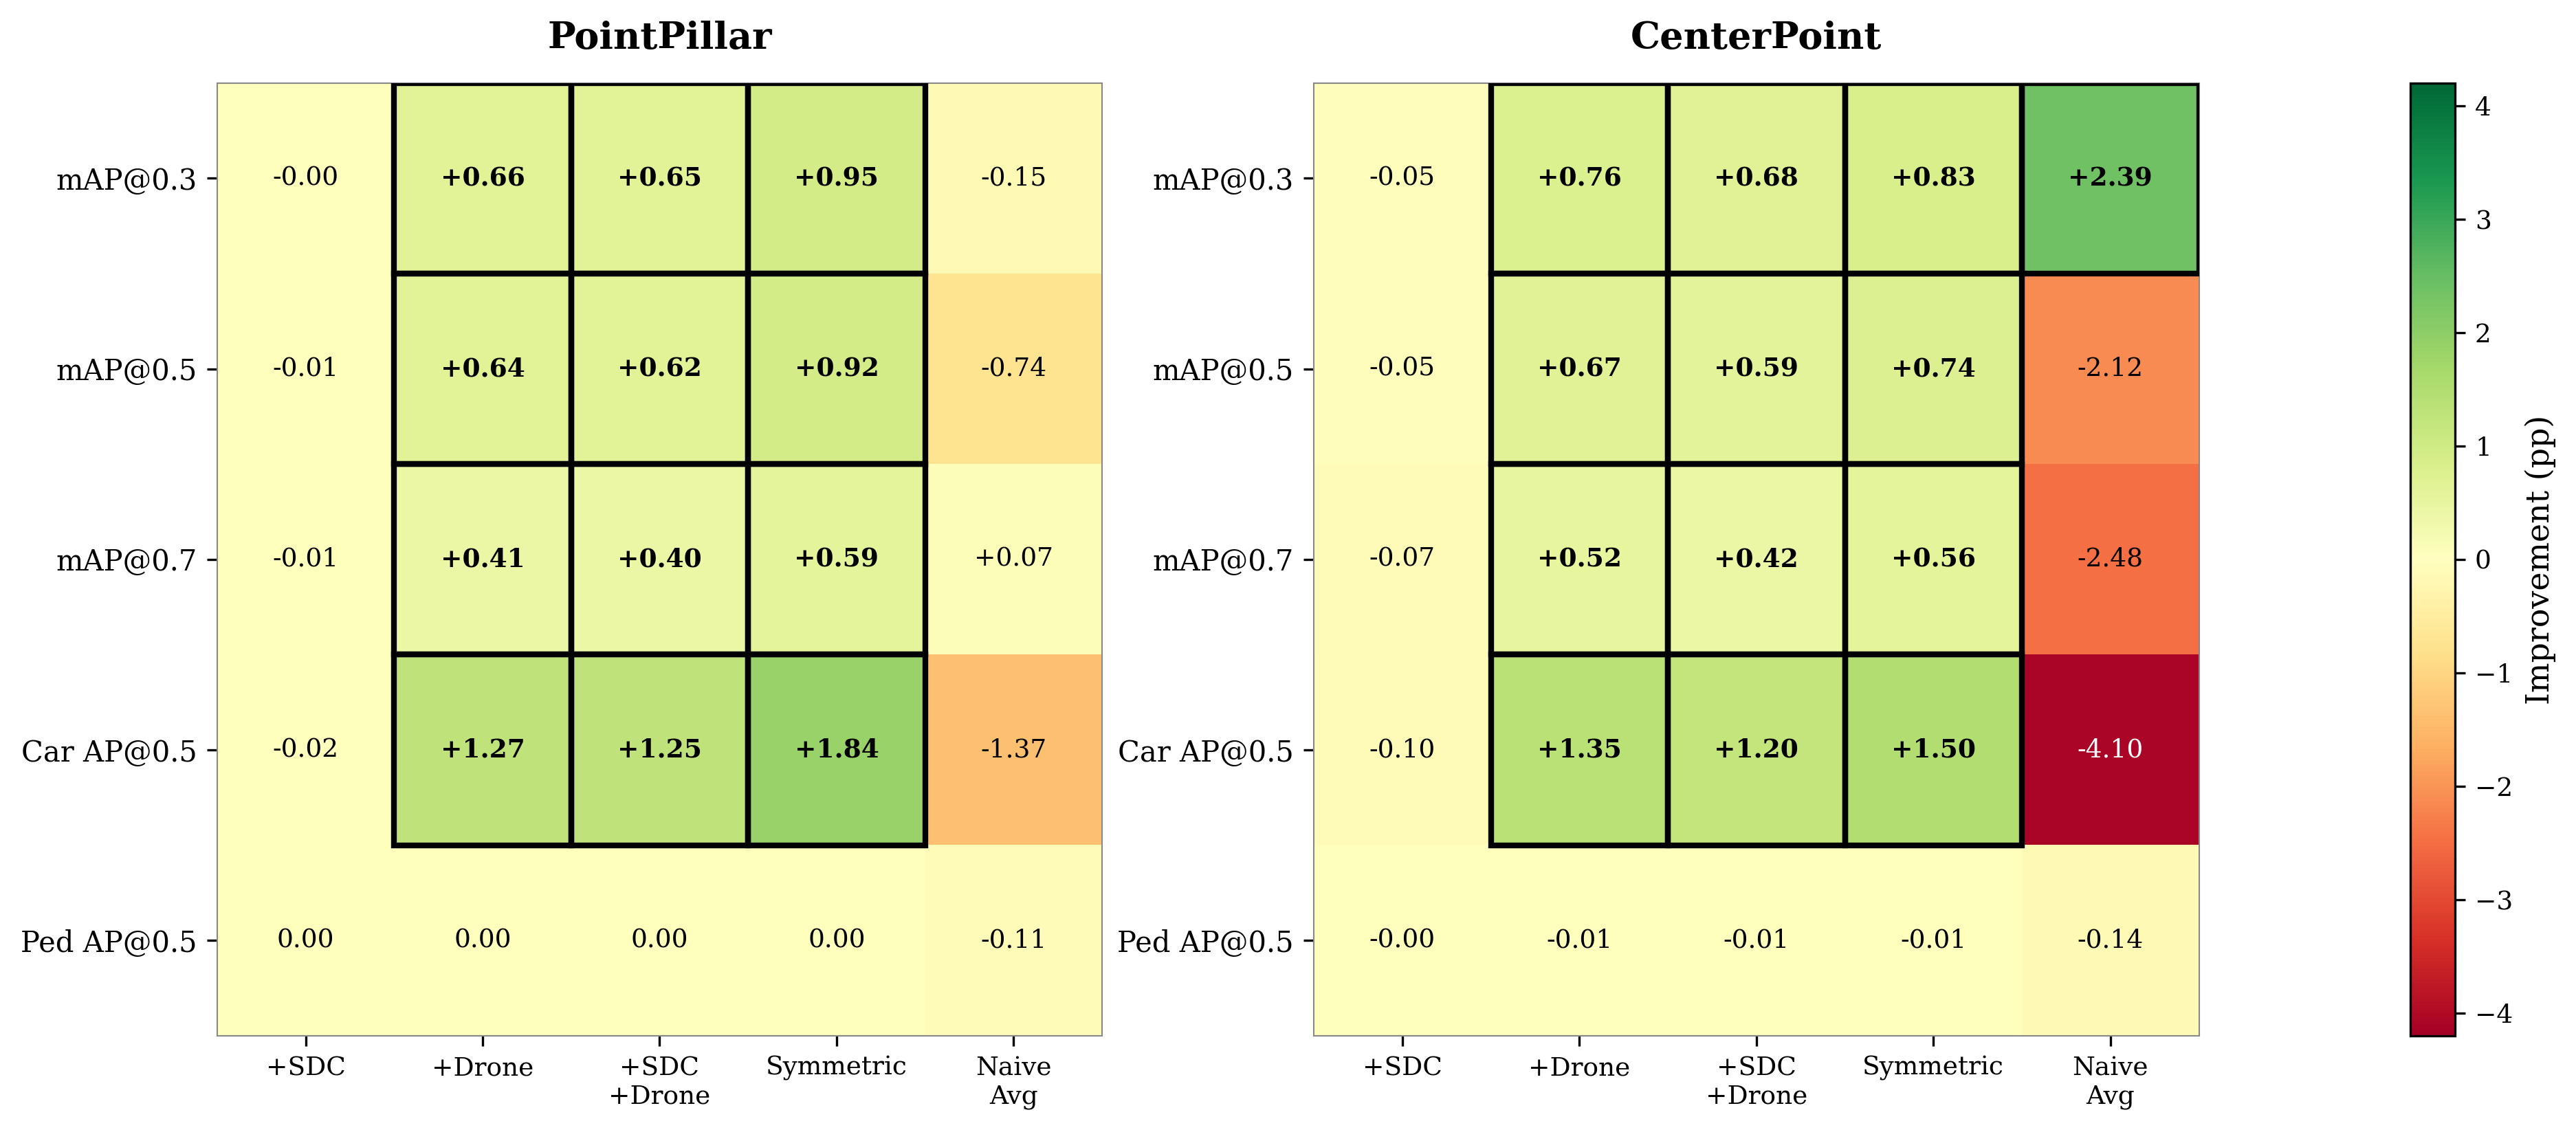
\includegraphics[width=0.85\textwidth]{fig4_improvement_heatmap.pdf}
\caption{Improvement over LiDAR-only baseline (percentage points) across all metrics and fusion configurations. Symmetric fusion shows the most consistent gains across all IoU thresholds. Naive averaging hurts at all thresholds. Cells with bold borders indicate statistical significance ($p < 0.001$).}\label{fig:heatmap}
\end{figure}

\begin{figure}[H]
\centering
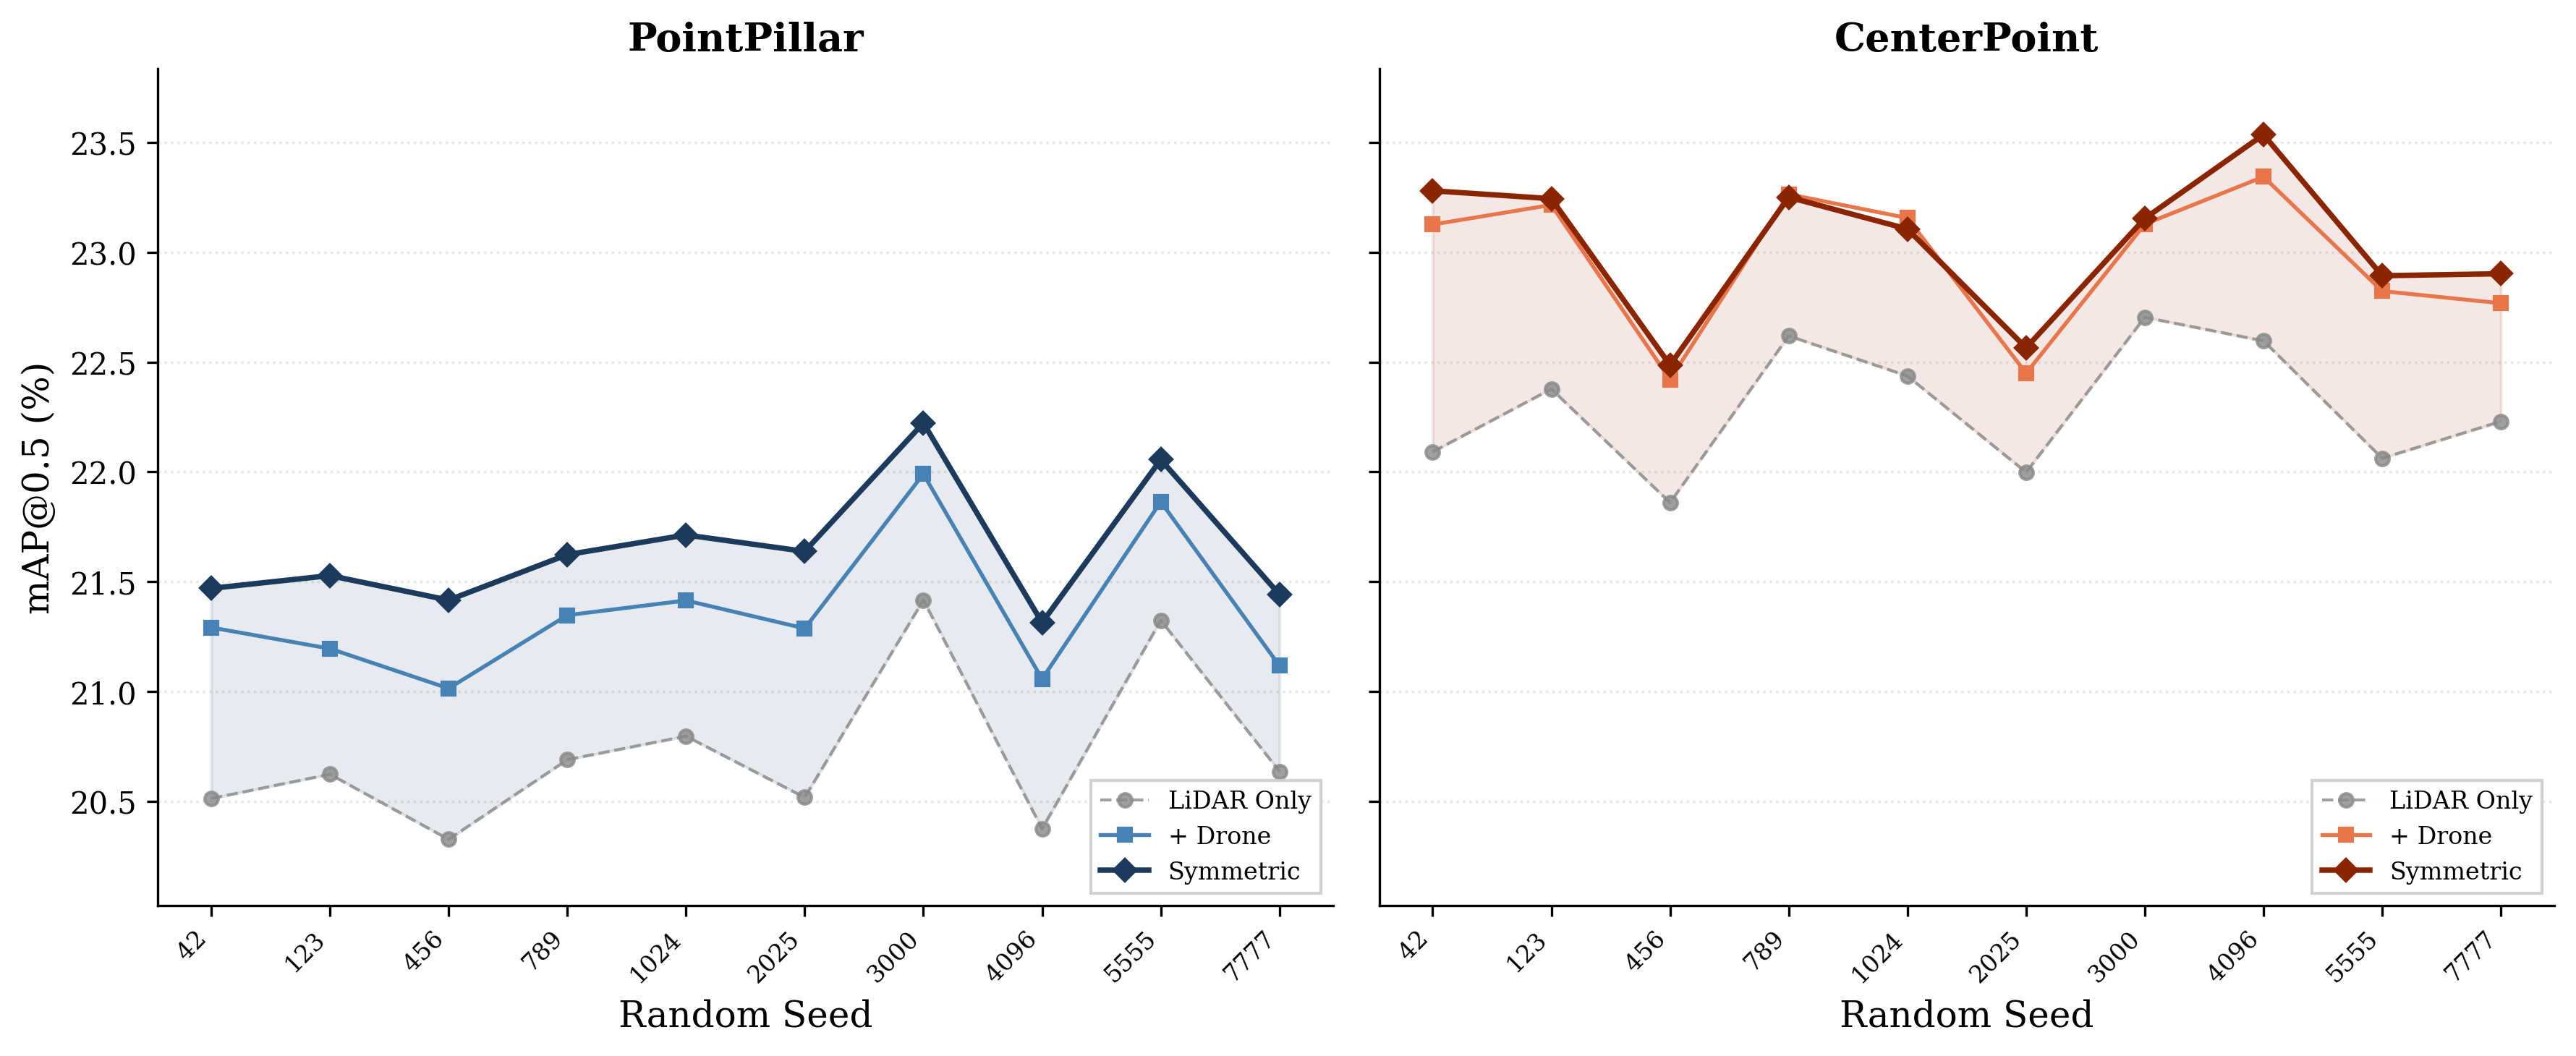
\includegraphics[width=0.75\textwidth]{fig3_per_seed_mAP05.pdf}
\caption{Per-seed mAP@0.5 consistency across 10 random seeds. Symmetric fusion (solid red) consistently outperforms the LiDAR-only baseline (dashed black), with no seed showing degradation. The narrow error bands reflect the stability afforded by the larger 2{,}600-frame dataset.}\label{fig:per_seed}
\end{figure}

\subsection{Qualitative Analysis}

Figure~\ref{fig:qualitative} provides a multi-view overview of fusion on a representative frame, and Figure~\ref{fig:fp_suppression} highlights the false positive suppression mechanism in detail.

\begin{figure}[H]
\centering
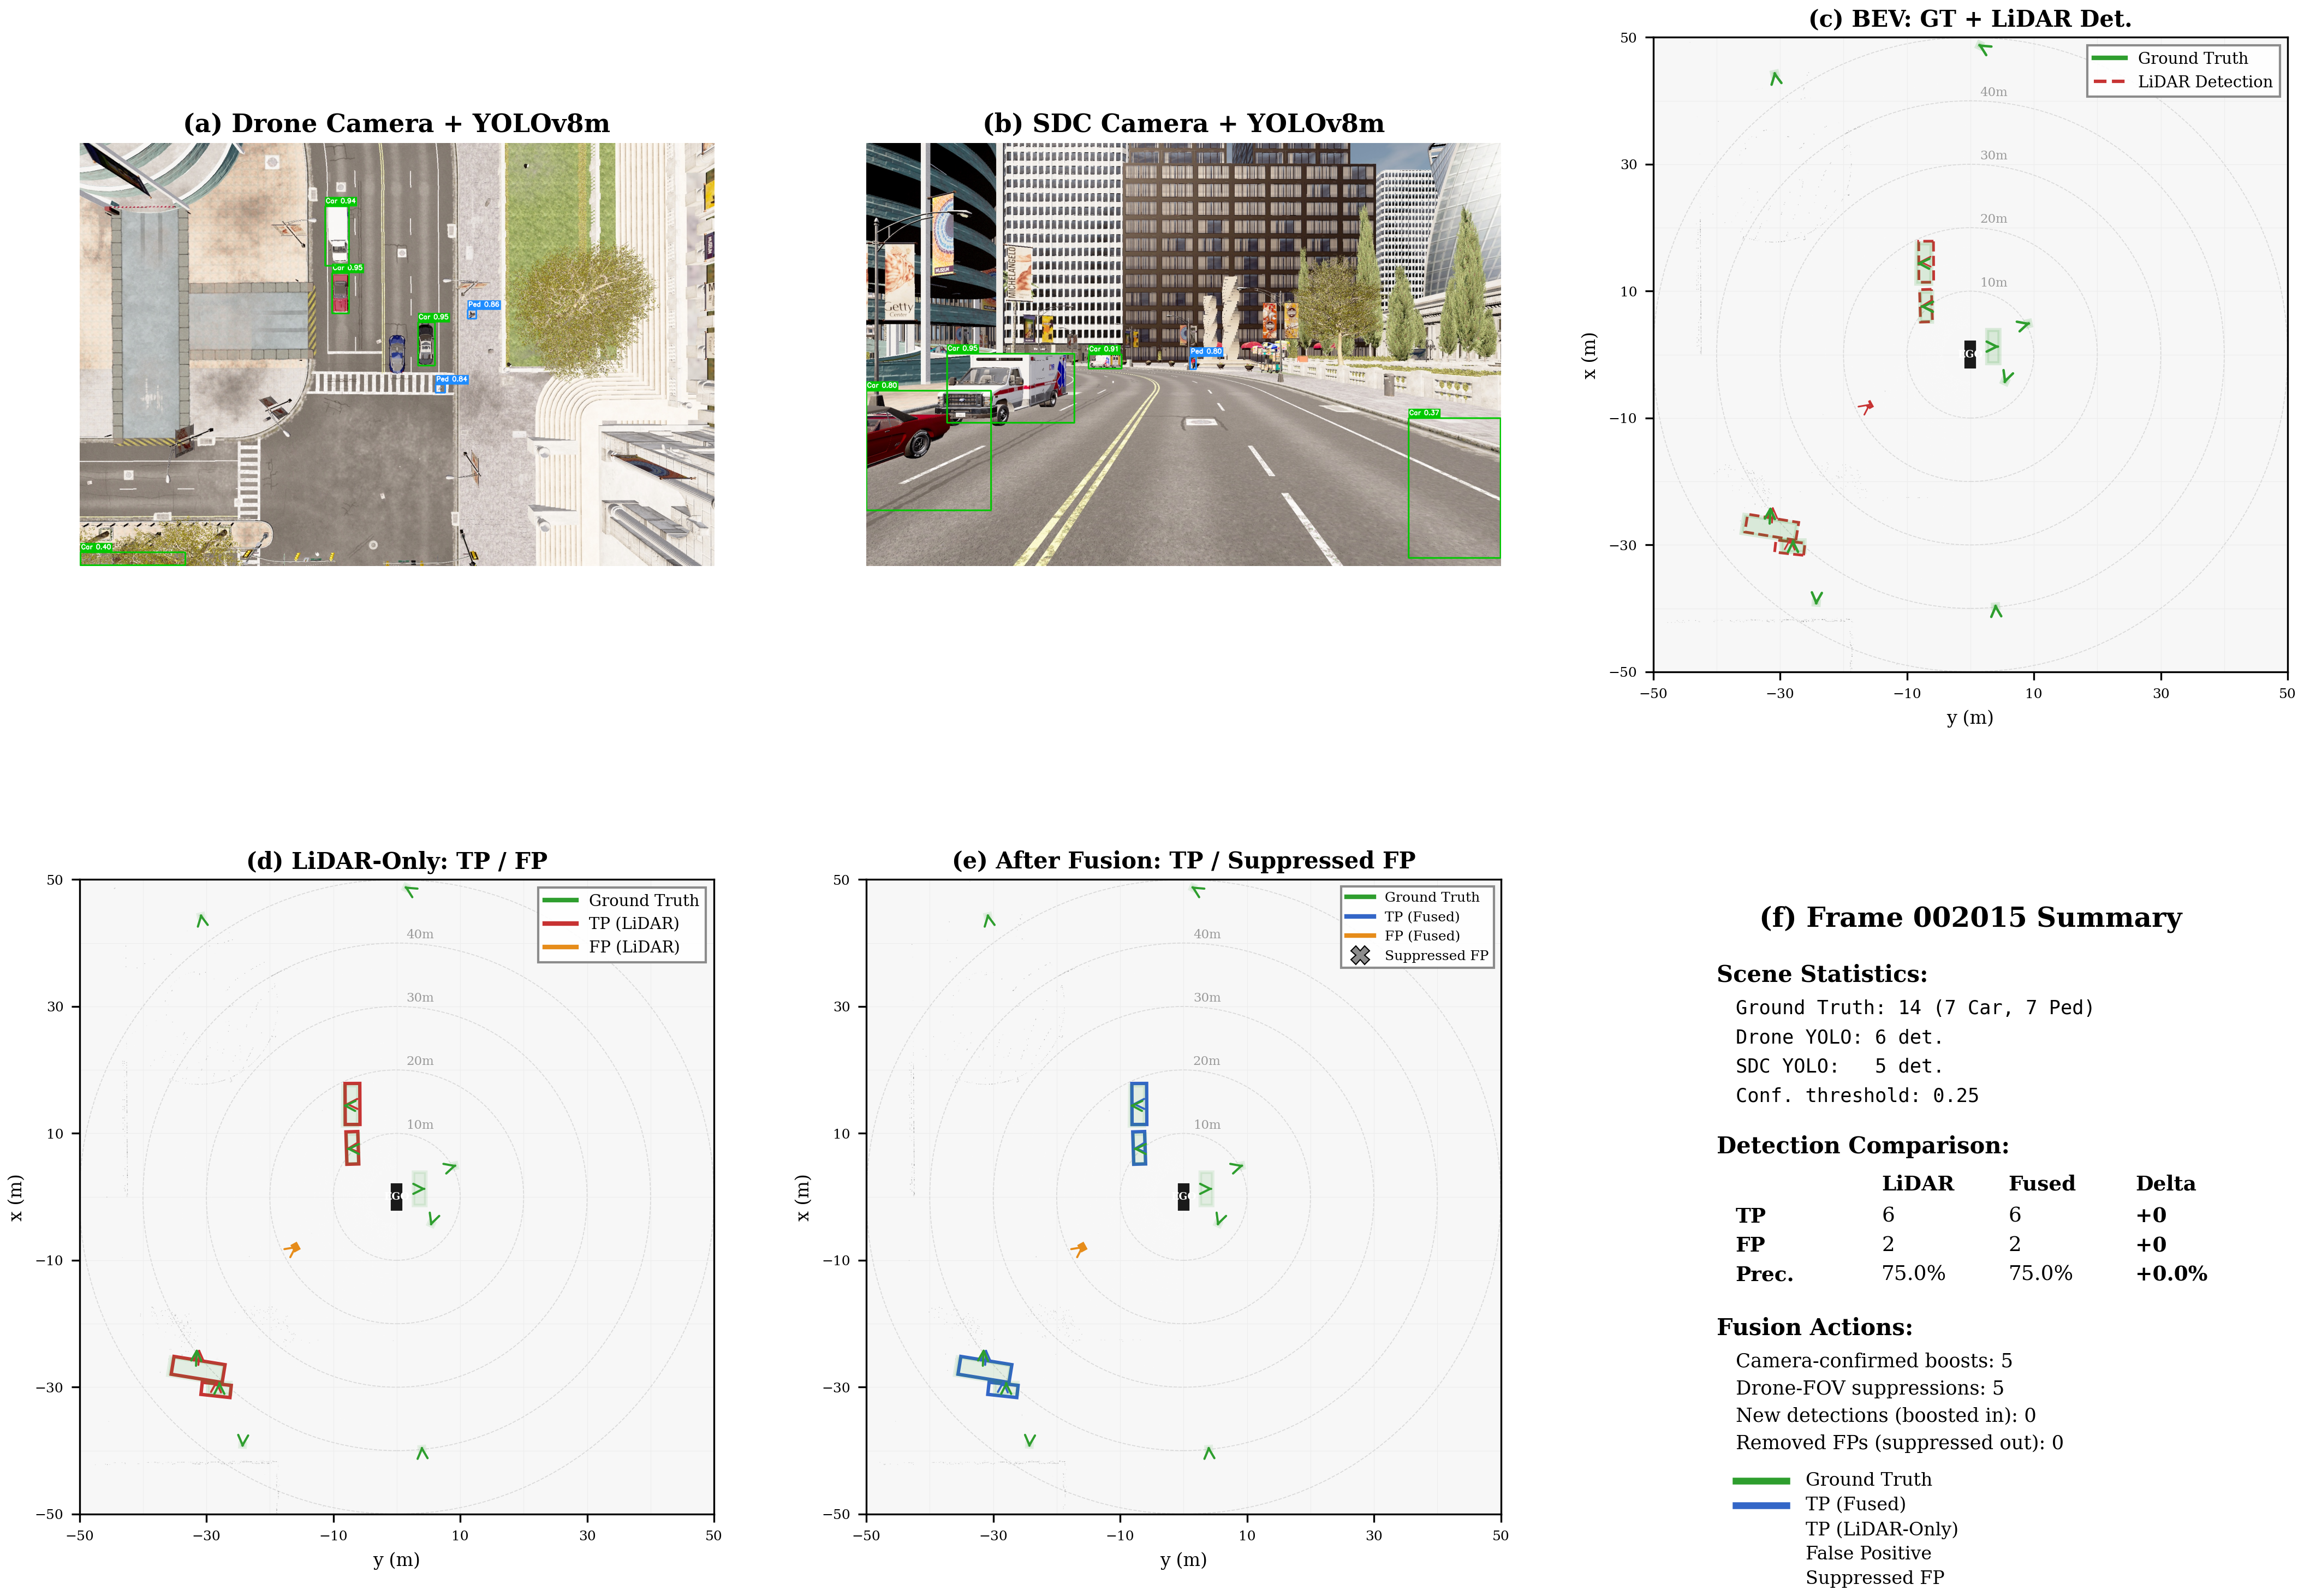
\includegraphics[width=0.95\textwidth]{fig_qualitative_overview.pdf}
\caption{Multi-view qualitative analysis (frame 002015, seed~0). \textbf{Top row:} (\textbf{a})~Drone camera with YOLOv8 detections, (\textbf{b})~SDC camera with YOLOv8 detections, (\textbf{c})~BEV showing ground-truth (green) and LiDAR detections (red dashed). \textbf{Bottom row:} (\textbf{d})~LiDAR-only true positives (red) and false positives (orange) vs.\ ground truth, (\textbf{e})~after fusion with camera-confirmed boosts, (\textbf{f})~summary statistics showing 5 camera-confirmed boosts with precision preserved at 75\%.}\label{fig:qualitative}
\end{figure}

\begin{figure}[H]
\centering
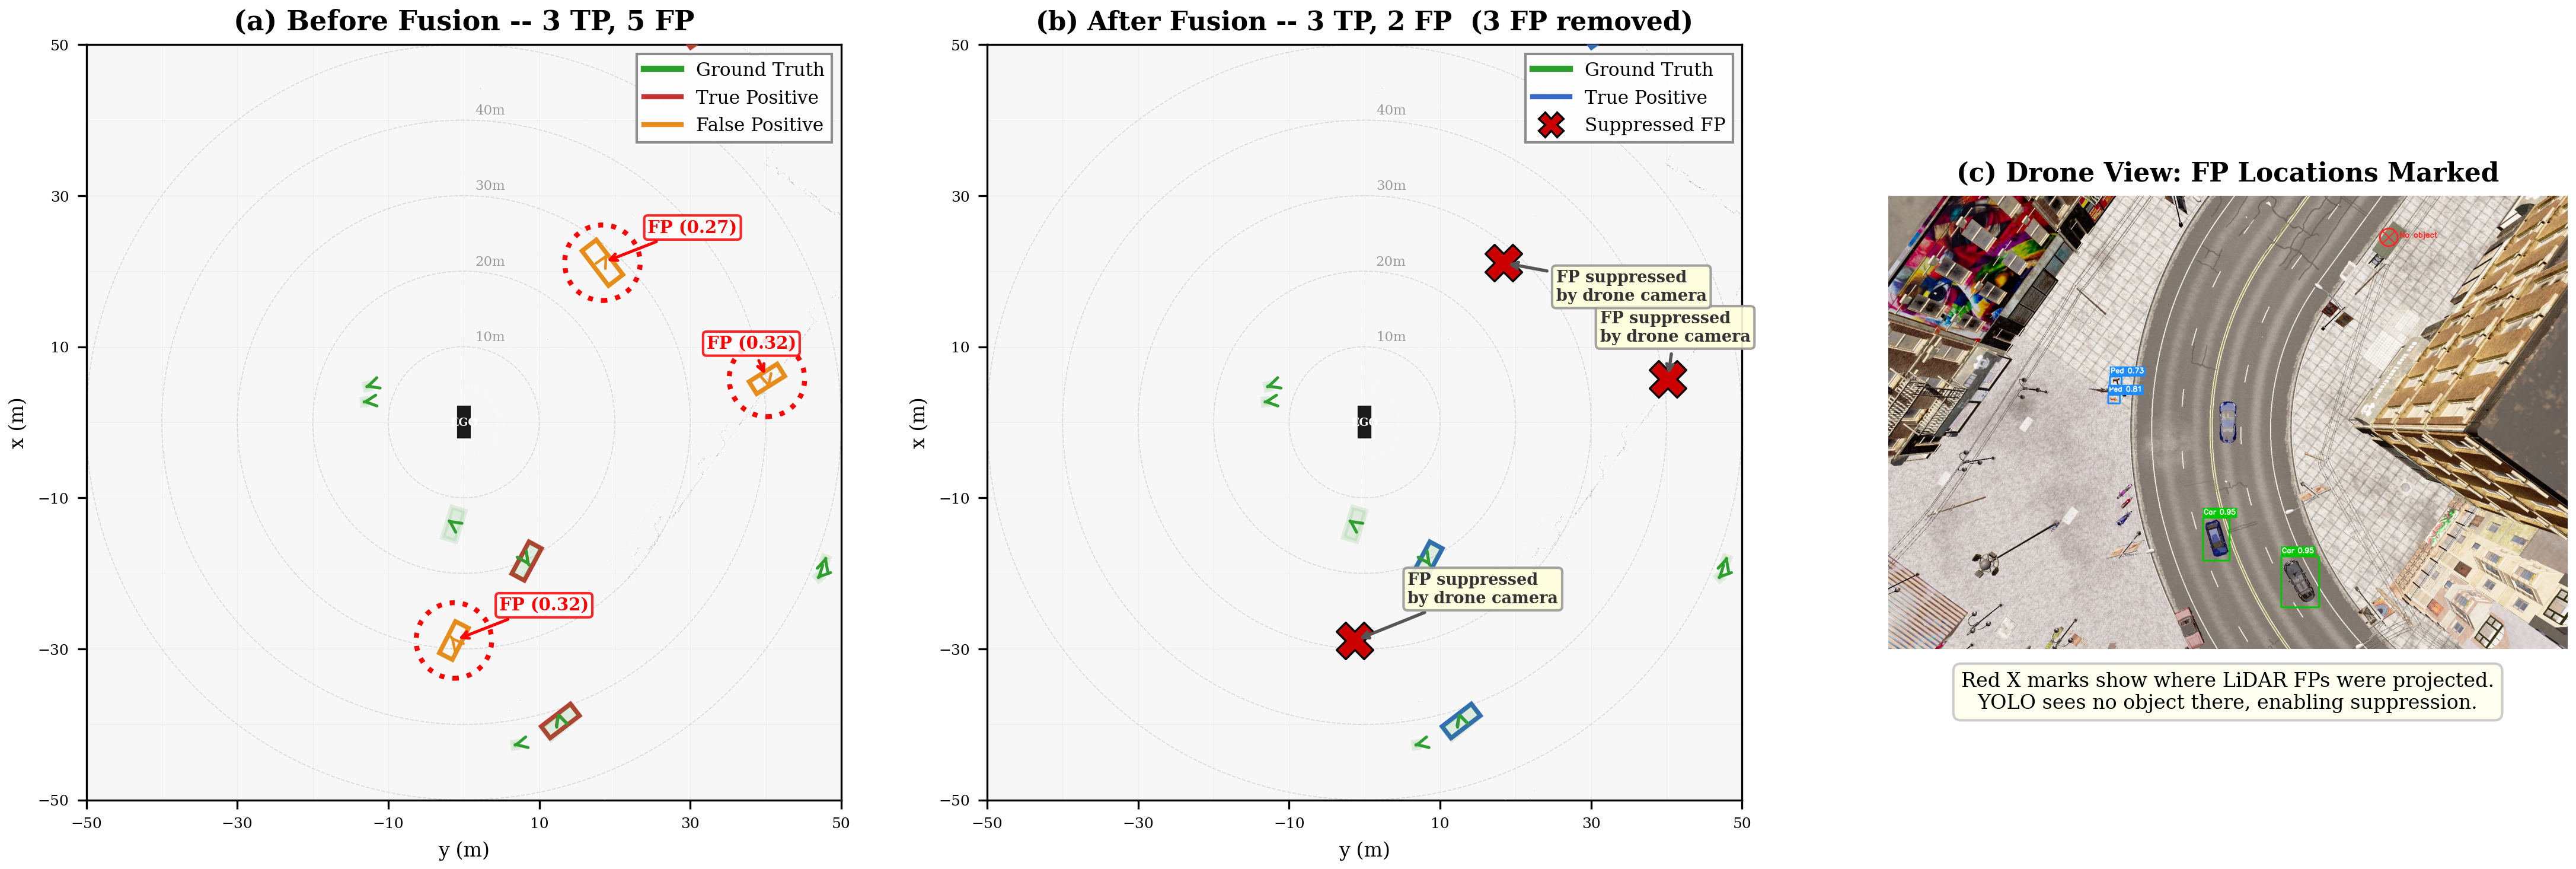
\includegraphics[width=0.95\textwidth]{fig_qualitative_fp_suppression.pdf}
\caption{False positive suppression example (frame 000213, seed~0). (\textbf{a})~Before fusion: 3 true positives and 5 false positives, with suppressible FPs circled in red with confidence scores. (\textbf{b})~After fusion: 3 FPs removed by the drone camera, shown as red crosses with annotation arrows. (\textbf{c})~Drone camera view with the FP locations projected---no objects exist at those positions, confirming the LiDAR detections as spurious.}\label{fig:fp_suppression}
\end{figure}

\subsection{Parameter Sensitivity Analysis}\label{sec:sensitivity}

To verify that the fusion improvements are not an artifact of specific hyper-parameter choices, we conduct a one-at-a-time sensitivity analysis by sweeping each fusion parameter across a wide range while holding the others at their defaults.  We use the symmetric fusion configuration (best performer) on the PointPillar seed-0 val split.  Figure~\ref{fig:sensitivity} summarizes the results.

\begin{figure}[H]
\centering
\includegraphics[width=0.95\textwidth]{fig_sensitivity.pdf}
\caption{Parameter sensitivity analysis (symmetric fusion, PointPillar seed~0). Each panel sweeps one parameter while others are held at their default values (red star).  The dashed line marks the LiDAR-only baseline.  \textbf{(a)}~Single-camera boost $\beta_{\mathrm{single}}$: negligible effect (range $<$0.02~pp).  \textbf{(b)}~Dual-camera boost $\beta_{\mathrm{dual}}$: negligible effect (range $<$0.06~pp).  \textbf{(c)}~Suppression factor $\gamma$: the dominant parameter; stronger suppression ($\gamma \to 0.5$) monotonically improves mAP, confirming FP removal as the primary mechanism.  \textbf{(d)}~Confidence gate $\theta_{\mathrm{low}}$: a clear threshold exists near 0.35; above this value the gate captures most suppressible FPs and performance saturates.  \textbf{(e)}~Matching IoU $\tau_{\mathrm{IoU}}$: nearly flat across the full range, indicating robustness to the matching criterion.}\label{fig:sensitivity}
\end{figure}

Three key findings emerge:

\begin{enumerate}[leftmargin=*,labelsep=4.9mm]
\item \textbf{Suppression factor $\gamma$ is the dominant parameter.}  Sweeping $\gamma$ from 0.50 (aggressive suppression) to 1.00 (no suppression) produces a monotonic decline in mAP from 21.88\% to 20.54\%.  At $\gamma = 1.0$, the system degenerates to the LiDAR-only baseline (20.56\%), confirming that FP suppression---not confidence boosting---drives the improvement.  Our default $\gamma = 0.75$ is a \emph{conservative} choice; stronger suppression ($\gamma \leq 0.65$) yields an additional +0.36~pp, indicating untapped potential.

\item \textbf{Boost factors have negligible impact.}  Both $\beta_{\mathrm{single}}$ (range 1.00--1.30) and $\beta_{\mathrm{dual}}$ (range 1.00--1.50) alter mAP by less than 0.06~pp.  This further confirms that the fusion benefit originates from the suppress branch, not from confidence amplification.

\item \textbf{The method is robust across all parameters.}  Across all 41 parameter configurations evaluated, \emph{every single setting} in which suppression is active ($\gamma < 1.0$ and $\theta_{\mathrm{low}} \geq 0.35$) improves over the LiDAR-only baseline.  There is no narrow ``sweet spot'' that could suggest overfitting to a particular parameter combination.
\end{enumerate}

%=================================================================
\section{Discussion}\label{sec:discussion}

\subsection{False Positive Suppression as the Primary Mechanism}

The most important finding of this study is that camera-LiDAR fusion improves 3D detection primarily through \emph{false positive suppression}, not through occlusion recovery or recall improvement. The drone camera reduces false positives by 13\% while preserving all true positives, improving precision by 3.1 percentage points. This finding has several implications:

\begin{enumerate}[leftmargin=*,labelsep=4.9mm]
\item \textbf{For system design:} The suppress mechanism is more valuable than the boost mechanism. Camera confirmation of existing LiDAR detections provides marginal improvement (boost alone achieves almost nothing, as shown by SDC-only results), but camera \emph{disconfirmation} of false detections is highly effective. The parameter sensitivity analysis (Section~\ref{sec:sensitivity}) provides independent confirmation: sweeping the boost factors $\beta$ across their entire range changes mAP by less than 0.06~pp, whereas sweeping the suppression factor $\gamma$ produces a 1.33~pp swing.

\item \textbf{For safety:} False positive reduction is arguably more important for practical deployment than recall improvement. Phantom detections trigger unnecessary braking (``phantom braking''), which reduces traffic efficiency, increases rear-end collision risk, and erodes passenger trust. A system that produces fewer false alarms is safer and more commercially viable.

\item \textbf{For precision-recall trade-off:} Late fusion operates on the precision side of the precision-recall trade-off. It cannot recover objects that the LiDAR completely fails to detect (recall-limited regime) but can effectively prune spurious detections (precision-limited regime). This suggests that late fusion is most valuable when the base detector has adequate recall but noisy confidence scores.
\end{enumerate}

\subsection{Symmetric vs. Asymmetric Fusion}

A surprising finding is that symmetric fusion (+0.92 pp) outperforms asymmetric dual-camera fusion (+0.63 pp) by +0.29 pp. In our preliminary study, we hypothesized that the SDC forward camera's narrow FOV would make it unsuitable for suppression: objects outside its FOV would be falsely penalized. In practice, the opposite occurs: the SDC camera effectively suppresses false positives within its frontal zone, and these frontal false positives are precisely where the drone camera is \emph{least} effective (because objects directly ahead of the vehicle are also visible from above, making the drone's suppress decision redundant for frontal objects but the SDC provides an independent confirmation/disconfirmation signal).

The failure of SDC boost-only (2/10 positive seeds) corroborates this: the forward camera's value lies \emph{entirely} in its ability to suppress false positives, not in boosting true positives. When restricted to boost-only operation, the SDC camera provides virtually no improvement because the LiDAR already detects frontal objects effectively.

This has practical implications for multi-camera fusion system design: even narrow-FOV cameras can contribute meaningfully through suppression, as long as the suppress operation is restricted to low-confidence detections within the camera's actual FOV (i.e., the camera must have actually ``looked'' at the region in question).

\subsection{Naive Averaging as a Cautionary Tale}

The consistent degradation from naive score averaging ($-$0.74 pp, 0/10 positive seeds) demonstrates that fusion is not simply a matter of combining scores. The LiDAR detector's confidence scores are calibrated relative to the evaluation threshold; averaging with camera scores (which have different scale and semantics) destroys this calibration. This result underscores the importance of structured fusion logic that respects the different characteristics of each sensor's output.

\subsection{Transportation Safety and Sustainability Implications}

From a sustainable transportation perspective, the false positive reduction mechanism has direct practical benefits:

\begin{itemize}[leftmargin=*,labelsep=5.8mm]
\item \textbf{Reduced phantom braking.} 62 false positives removed from the evaluation set correspond to 62 potential phantom braking events that would reduce traffic flow and increase fuel consumption. At highway speeds, each phantom braking event can trigger a cascade of slowdowns affecting following vehicles.
\item \textbf{Smoother traffic flow.} A perception system with higher precision produces smoother planning trajectories, reducing the stop-and-go patterns that maximize fuel consumption and emissions.
\item \textbf{Improved trust.} False positive reduction improves the human rider's experience and trust in autonomous systems, supporting public acceptance of autonomous mobility---a prerequisite for the transportation efficiency gains that autonomous vehicles promise.
\item \textbf{Cost-effective safety.} The proposed approach uses inexpensive cameras (potentially on existing traffic infrastructure or lightweight drones) to improve a LiDAR-based perception system without replacing or upgrading the LiDAR itself, offering a sustainable pathway to enhanced safety.
\end{itemize}

\noindent\textbf{Practical deployment context.}
While a dedicated drone hovering above each vehicle is impractical for mass-market autonomous driving, the overhead camera in this study serves as a \emph{proxy for elevated infrastructure cameras} in Vehicle-to-Everything (V2X) cooperative perception deployments.
Fixed pole- or building-mounted cameras at intersections and roundabouts---actively being deployed under ETSI C-ITS and SAE V2X standards in cities such as Singapore, Shanghai, and several European smart-corridor pilots---provide a comparable top-down field of view.
Our results quantify the detection benefit of such infrastructure: a single elevated camera reduces LiDAR false positives by 13\% through the same suppress mechanism demonstrated here, providing empirical justification for V2X perception investment.
The fusion framework is architecture-agnostic; replacing the drone feed with a roadside-unit (RSU) camera feed requires only an updated extrinsic calibration matrix, with no changes to the boost/suppress logic.

\subsection{Comparison Across IoU Thresholds}

The fusion improvements are consistent across IoU thresholds: symmetric fusion achieves +0.95 pp at IoU 0.3, +0.92 pp at IoU 0.5, and +0.59 pp at IoU 0.7. The improvement at IoU 0.7 (+3.6\% relative) is proportionally similar to IoU 0.5 (+4.4\%), indicating that the fusion benefit extends to strictly localized detections. This contrasts with our preliminary finding that IoU 0.7 showed ``minimal improvement''---the larger dataset and more seeds reveal that the improvement is real but smaller in absolute terms.

\subsection{Limitations and Future Work}

Several limitations motivate future research:

\begin{itemize}[leftmargin=*,labelsep=5.8mm]
\item \textbf{Simulation-only evaluation.} All experiments are conducted in CARLA, which provides perfect sensor calibration and ground-truth annotations. Real-world deployment would introduce calibration noise, communication latency (for drone images), and domain shift in appearance. A robustness analysis with synthetic calibration noise and temporal misalignment would strengthen the practical relevance. Future work should evaluate sim-to-real transfer~\cite{yue2019domain} and real-world drone-vehicle cooperative scenarios.

\item \textbf{Pedestrian detection remains weak.} Pedestrian AP@0.5 (2.69\%) is near-zero across all configurations, and the fusion provides no improvement for pedestrians. This reflects the inherent difficulty of detecting small, sparse-point objects from LiDAR alone. Deep fusion approaches that incorporate camera appearance features may be necessary to meaningfully improve pedestrian detection.

\item \textbf{Hand-tuned fusion parameters.} Although the sensitivity analysis (Section~\ref{sec:sensitivity}) demonstrates robustness across a wide parameter range, the fusion hyper-parameters are still selected manually rather than learned from data. End-to-end parameter learning (e.g., via CLOCs-style fusion networks~\cite{pang2020clocs}) could further improve performance and adapt the suppress/boost trade-off to different sensor geometries or scene densities.

\item \textbf{Static drone assumption.} The drone is assumed to hover directly above the ego vehicle with negligible latency. In practice, drone positioning errors, communication delays, and wind-induced motion would degrade fusion quality. Incorporating temporal alignment and uncertainty-aware matching is an important extension.

\item \textbf{Two-class limitation.} The current evaluation covers only \texttt{Car} and \texttt{Pedestrian} classes. Extending to additional classes (e.g., \texttt{Cyclist}, \texttt{Truck}) and evaluating on larger, more diverse datasets (e.g., nuScenes~\cite{caesar2020nuscenes}, Waymo~\cite{sun2020waymo}) would strengthen the generalizability claims.

\item \textbf{Late fusion ceiling.} Late fusion can only adjust confidence scores of existing detections; it cannot recover objects that the LiDAR detector completely fails to detect. Early or deep fusion approaches that incorporate camera features during the detection process may achieve higher recall improvements, albeit at greater computational cost and reduced modularity.
\end{itemize}

%=================================================================
\section{Conclusions}\label{sec:conclusions}

This paper presented a dual-camera LiDAR fusion framework for 3D object detection in urban driving environments, with systematic comparison of asymmetric, symmetric, and naive-averaging fusion strategies. The key contributions and findings are:

\begin{enumerate}[leftmargin=*,labelsep=4.9mm]
\item \textbf{Symmetric fusion outperforms asymmetric.} Contrary to the intuition that narrow-FOV cameras should be restricted to boost-only operations, we find that symmetric fusion---where both cameras apply boost and suppress---achieves the best performance (+0.92 pp mAP@0.5, +4.4\% relative, sign test $p = 0.001$, $t$-test $p < 0.0001$). The SDC forward camera's value lies entirely in its suppression capability, not in boosting.

\item \textbf{False positive suppression is the primary mechanism.} The drone camera reduces false positives by 13\% while preserving all true positives, improving precision from 66.1\% to 69.2\%. This finding reframes camera-LiDAR fusion as a \emph{precision improvement} tool rather than a recall recovery mechanism in the late-fusion regime.

\item \textbf{Strong statistical significance.} Ten-seed validation with both parametric ($t$-test $p < 0.0001$) and non-parametric (sign test $p = 0.001$) tests provides compelling evidence that the fusion improvement is both consistent and statistically reliable. The larger dataset (2{,}600 frames) substantially reduces cross-seed variance.

\item \textbf{Dual-detector validation.} The fusion framework is evaluated with both PointPillar and CenterPoint. CenterPoint achieves a higher baseline (22.30\% vs.\ 20.76\% mAP@0.5) yet exhibits a nearly identical fusion gain: symmetric fusion improves CenterPoint by +0.74 pp (+3.3\%), with 10/10 positive seeds ($p = 0.001$). This confirms that the late-fusion benefit is detector-agnostic and generalizes across anchor-based and anchor-free architectures.

\item \textbf{Practical and modular framework.} The late-fusion approach requires no retraining of the base detectors, adds negligible computational overhead, and is agnostic to the specific 3D and 2D detection architectures used.
\end{enumerate}

From a sustainable transportation perspective, false positive suppression translates directly to smoother autonomous driving with fewer phantom braking events, supporting improved traffic flow and reduced emissions. The cost-effective nature of the approach---using inexpensive cameras to refine existing LiDAR perception---aligns with sustainable smart-city transportation strategies.

Within the scope of this simulation study, these results suggest two principles for autonomous driving perception: (1) cameras at \emph{complementary} viewpoints (e.g., overhead) provide the greatest fusion benefit, consistent with the intuition that viewpoint diversity resolves ambiguities that viewpoint redundancy cannot; and (2) even narrow-FOV cameras contribute meaningfully through \emph{false positive suppression}, provided the fusion logic respects each camera's coverage boundaries. Validating these principles on real-world data and across additional detector architectures is an important direction for future work.

%%%%%%%%%%%%%%%%%%%%%%%%%%%%%%%%%%%%%%%%%%

\vspace{6pt}

%%%%%%%%%%%%%%%%%%%%%%%%%%%%%%%%%%%%%%%%%%
\authorcontributions{Conceptualization, X.Z.\ and C.A.; methodology, X.Z.; software, X.Z.; validation, X.Z.; formal analysis, X.Z.; investigation, X.Z.; resources, C.A.; data curation, X.Z.; writing---original draft preparation, X.Z.; writing---review and editing, X.Z.\ and C.A.; visualization, X.Z.; supervision, C.A.; project administration, C.A. All authors have read and agreed to the published version of the manuscript.}

%%%%%%%%%%%%%%%%%%%%%%%%%%%%%%%%%%%%%%%%%%
\funding{This research received no external funding.}

%%%%%%%%%%%%%%%%%%%%%%%%%%%%%%%%%%%%%%%%%%
\acknowledgments{The authors acknowledge the use of the CARLA simulator for data collection and the OpenPCDet framework for LiDAR detection experiments. Computational resources were provided by Concordia University.}

%%%%%%%%%%%%%%%%%%%%%%%%%%%%%%%%%%%%%%%%%%
\conflictsofinterest{The authors declare no conflict of interest.}

%%%%%%%%%%%%%%%%%%%%%%%%%%%%%%%%%%%%%%%%%%
\paragraph{Data and Code Availability} The data collection scripts, fusion evaluation code, and trained model configurations will be made available at \url{https://github.com/Jynxzzz/dual-camera-lidar-fusion} upon publication.

%%%%%%%%%%%%%%%%%%%%%%%%%%%%%%%%%%%%%%%%%%
\abbreviations{The following abbreviations are used in this manuscript:\\

\noindent
\begin{tabular}{@{}ll}
AP & Average Precision\\
BEV & Bird's-Eye View\\
FOV & Field of View\\
FP & False Positive\\
FPN & Feature Pyramid Network\\
IoU & Intersection over Union\\
mAP & Mean Average Precision\\
SDC & Subject Driving Car\\
SSD & Single Shot Detector\\
TP & True Positive\\
UAV & Unmanned Aerial Vehicle\\
V2I & Vehicle-to-Infrastructure\\
V2X & Vehicle-to-Everything
\end{tabular}}

%%%%%%%%%%%%%%%%%%%%%%%%%%%%%%%%%%%%%%%%%%
\reftitle{References}

\externalbibliography{yes}
\bibliography{references}

%%%%%%%%%%%%%%%%%%%%%%%%%%%%%%%%%%%%%%%%%%
\end{document}
